\documentclass[]{article}
\usepackage[T1]{fontenc}
\usepackage{lmodern}
\usepackage{amssymb,amsmath}
\usepackage{ifxetex,ifluatex}
\usepackage{fixltx2e} % provides \textsubscript
% Set line spacing
% use upquote if available, for straight quotes in verbatim environments
\IfFileExists{upquote.sty}{\usepackage{upquote}}{}
\ifnum 0\ifxetex 1\fi\ifluatex 1\fi=0 % if pdftex
  \usepackage[utf8]{inputenc}
\else % if luatex or xelatex
  \ifxetex
    \usepackage{mathspec}
    \usepackage{xltxtra,xunicode}
  \else
    \usepackage{fontspec}
  \fi
  \defaultfontfeatures{Mapping=tex-text,Scale=MatchLowercase}
  \newcommand{\euro}{€}
\fi
% use microtype if available
\IfFileExists{microtype.sty}{\usepackage{microtype}}{}
\usepackage[margin=1in]{geometry}
\usepackage{graphicx}
% Redefine \includegraphics so that, unless explicit options are
% given, the image width will not exceed the width of the page.
% Images get their normal width if they fit onto the page, but
% are scaled down if they would overflow the margins.
\makeatletter
\def\ScaleIfNeeded{%
  \ifdim\Gin@nat@width>\linewidth
    \linewidth
  \else
    \Gin@nat@width
  \fi
}
\makeatother
\let\Oldincludegraphics\includegraphics
{%
 \catcode`\@=11\relax%
 \gdef\includegraphics{\@ifnextchar[{\Oldincludegraphics}{\Oldincludegraphics[width=\ScaleIfNeeded]}}%
}%
\ifxetex
  \usepackage[setpagesize=false, % page size defined by xetex
              unicode=false, % unicode breaks when used with xetex
              xetex]{hyperref}
\else
  \usepackage[unicode=true]{hyperref}
\fi
\hypersetup{breaklinks=true,
            bookmarks=true,
            pdfauthor={},
            pdftitle={Analysis Change of the Velopass data: the Bird's Eye View},
            colorlinks=true,
            citecolor=blue,
            urlcolor=blue,
            linkcolor=magenta,
            pdfborder={0 0 0}}
\urlstyle{same}  % don't use monospace font for urls
\setlength{\parindent}{0pt}
\setlength{\parskip}{6pt plus 2pt minus 1pt}
\setlength{\emergencystretch}{3em}  % prevent overfull lines
\setcounter{secnumdepth}{0}

%%% Change title format to be more compact
\usepackage{titling}
\setlength{\droptitle}{-2em}
  \title{Analysis Change of the Velopass data: the Bird's Eye View}
  \pretitle{\vspace{\droptitle}\centering\huge}
  \posttitle{\par}
  \author{}
  \preauthor{}\postauthor{}
  \date{}
  \predate{}\postdate{}




\begin{document}

\maketitle


\section{Introduction}\label{introduction}

We look at the higher level properties of the Velopass data.

\section{Data}\label{data}

We have written the data into files on the disk, and read them from
there,

Once read, we have to convert the dates to date/time objects.

\section{Usage over time}\label{usage-over-time}

How has the usage changed over time? Lets count the number of trips made
every day.

The data frame \emph{tripsByDay} contains three columns,

\begin{verbatim}
##          day num.trips dayOfWeek weekdayOrEnd
## 1 2010-01-04         5    Monday      weekday
## 2 2010-01-05         3   Tuesday      weekday
## 3 2010-01-06         6 Wednesday      weekday
## 4 2010-01-07         1  Thursday      weekday
## 5 2010-01-08         6    Friday      weekday
## 6 2010-01-09         1  Saturday      weekend
\end{verbatim}

We can plot the number of trips made on each day of the week, over the
duration of the data set

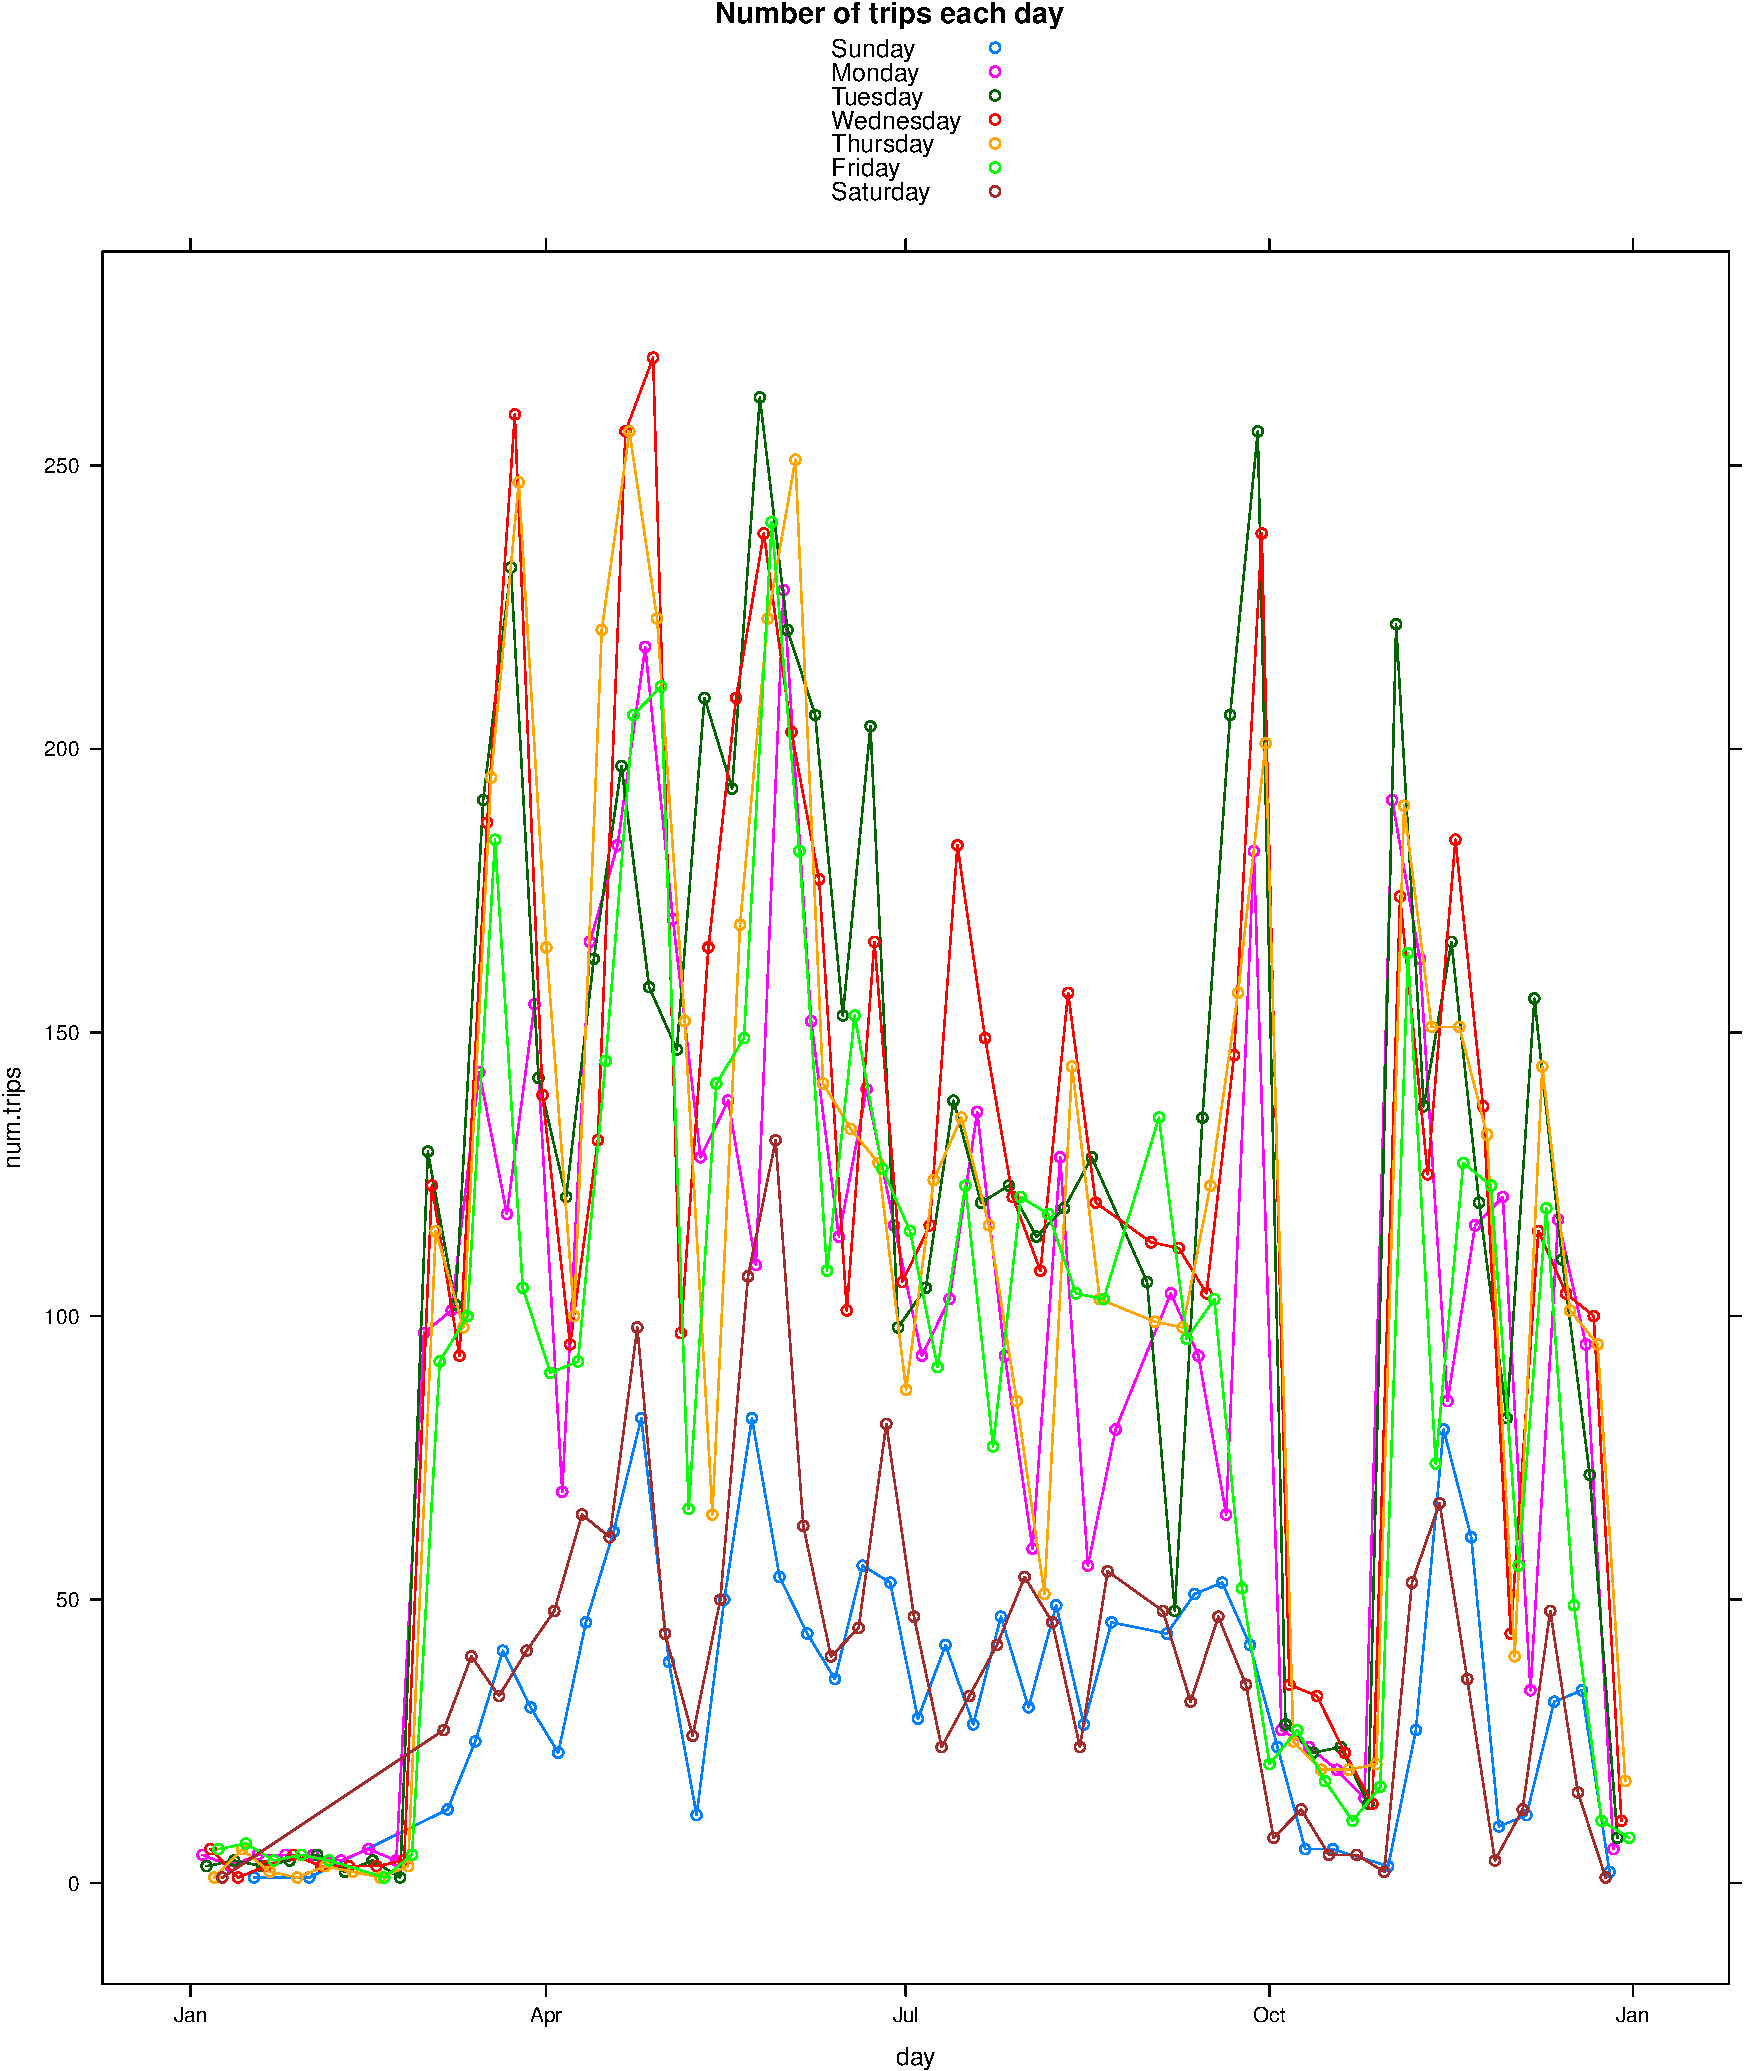
\includegraphics{velopassBirdsEye_files/figure-latex/plottripsbyday-1.pdf}
Since people's activity patterns change between the weekdays and
weekends, we can aggregate a week's days into these two categories,

\begin{figure}[htbp]
\centering
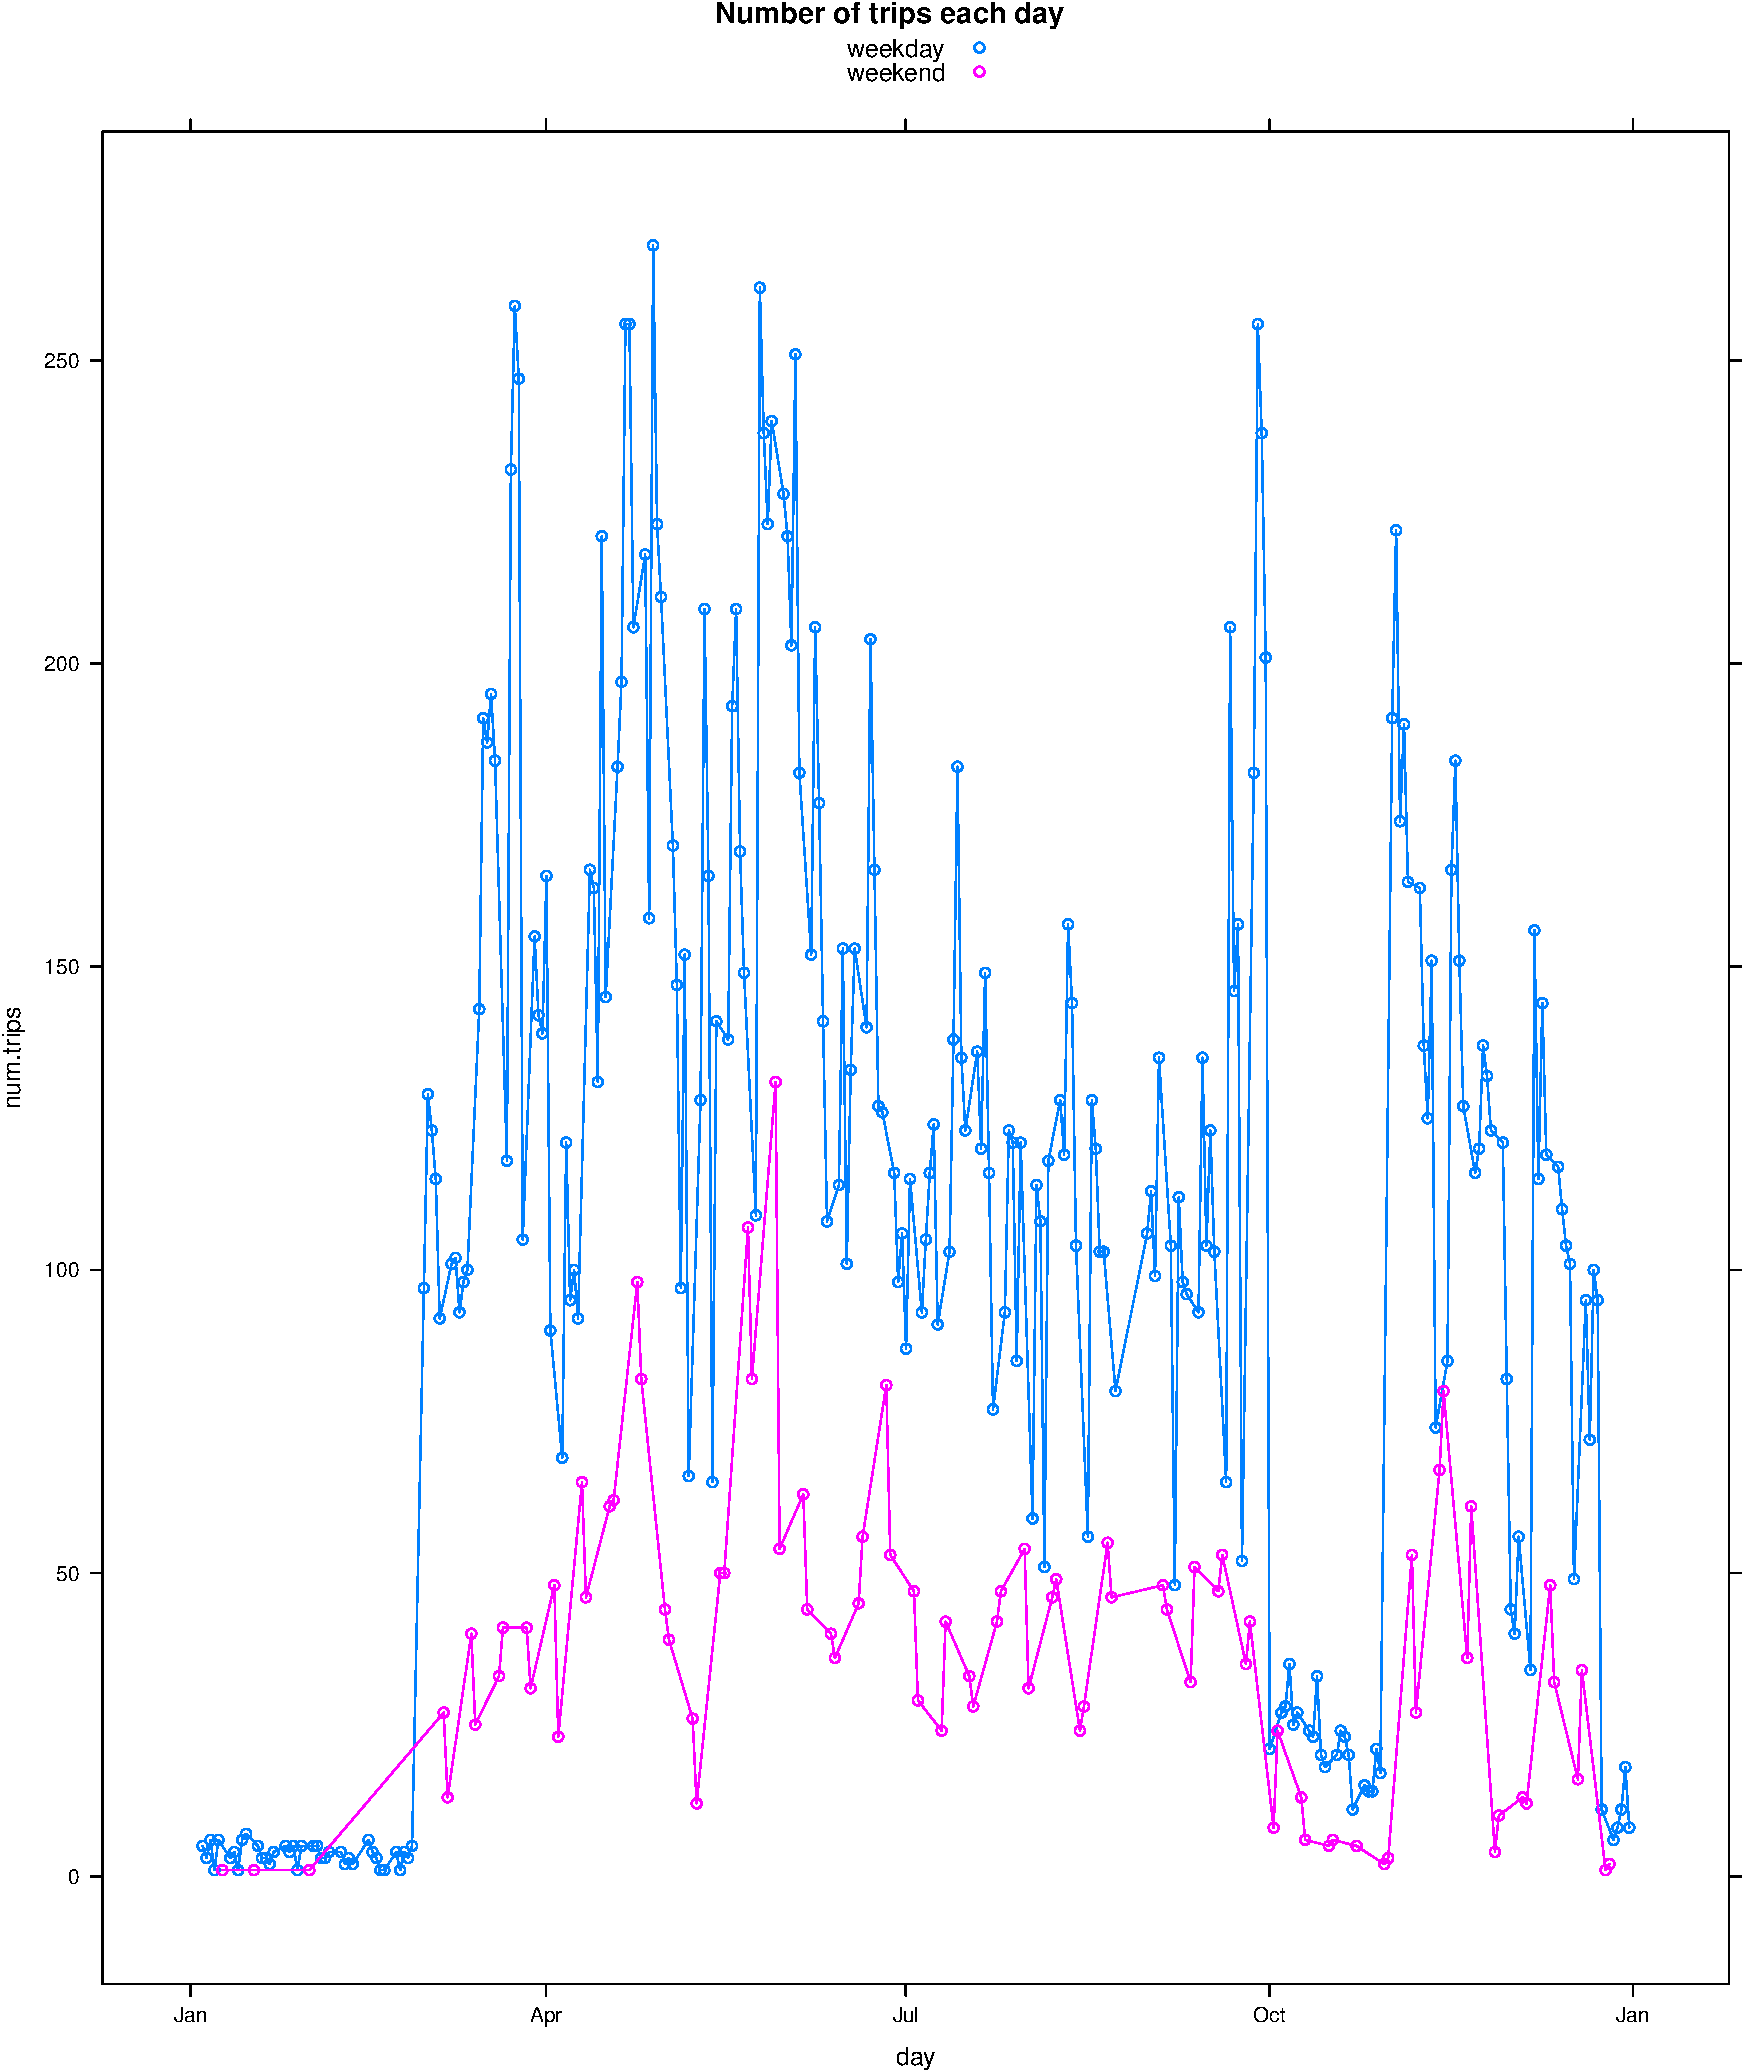
\includegraphics{velopassBirdsEye_files/figure-latex/plottripsweekdayend-1.pdf}
\caption{}
\end{figure}

We can add a column for the week during which the trip was made, and
look at the number of trips by week of the year.

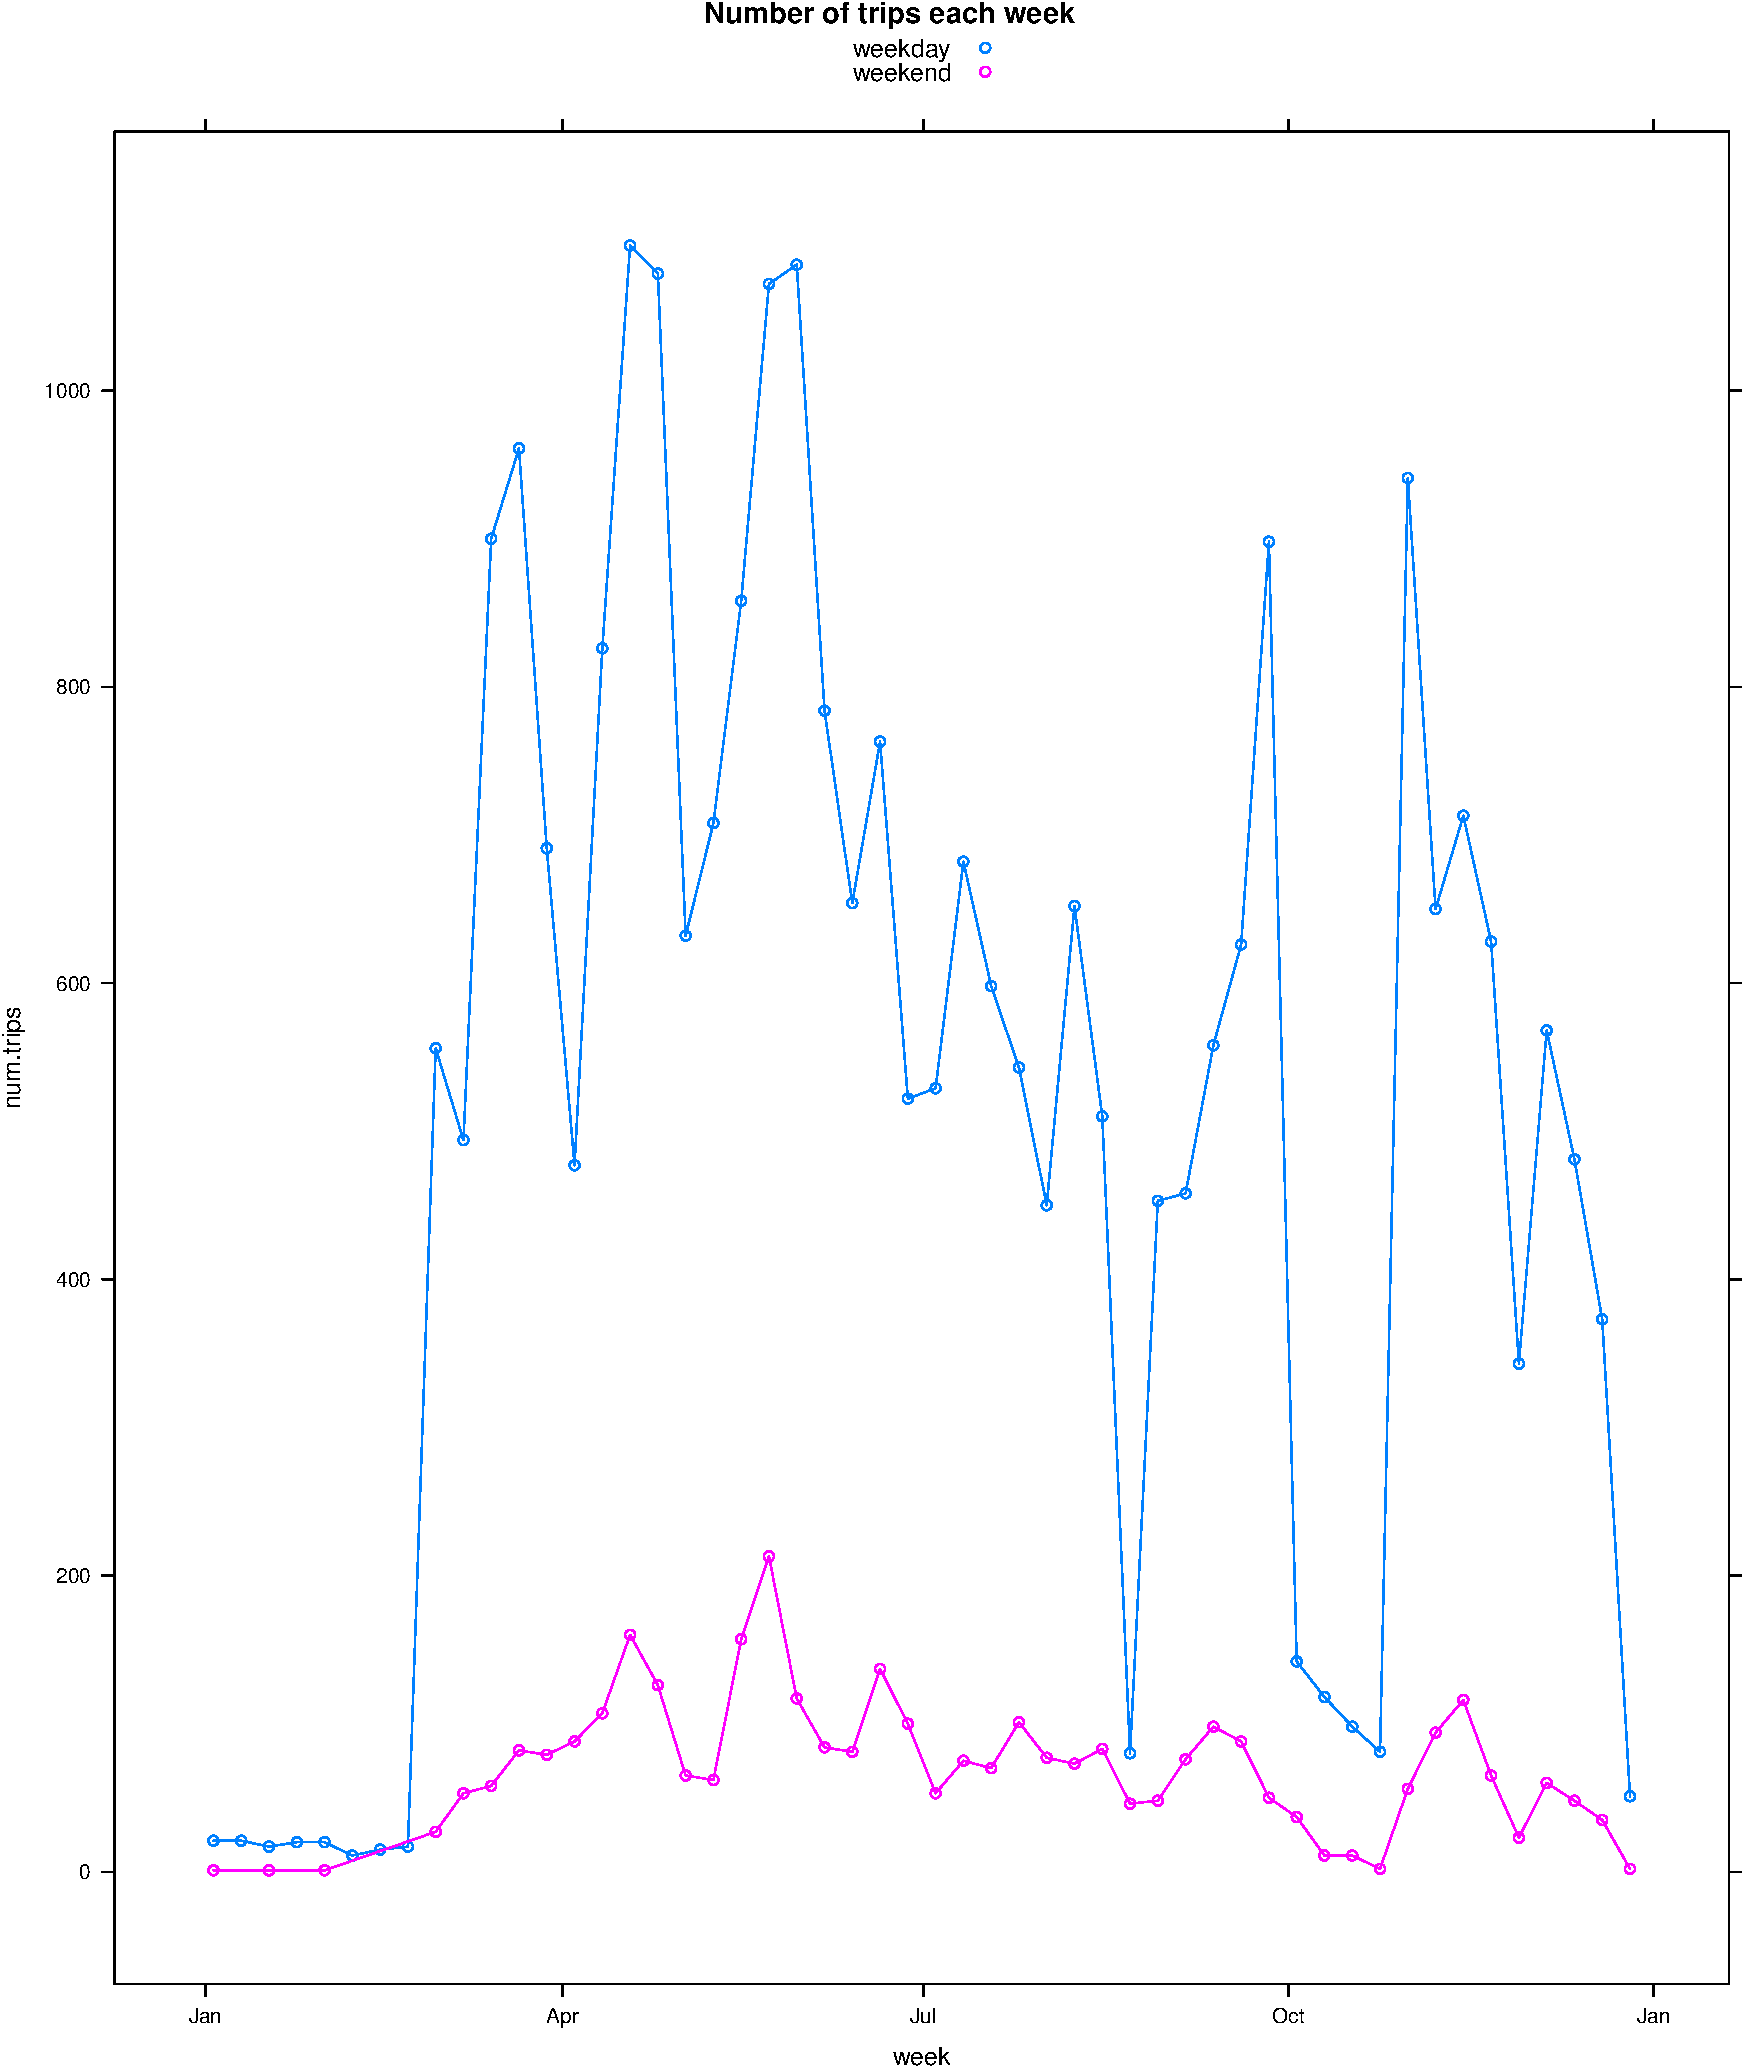
\includegraphics{velopassBirdsEye_files/figure-latex/tripsbyweek-1.pdf}
And do the same by month.

\begin{figure}[htbp]
\centering
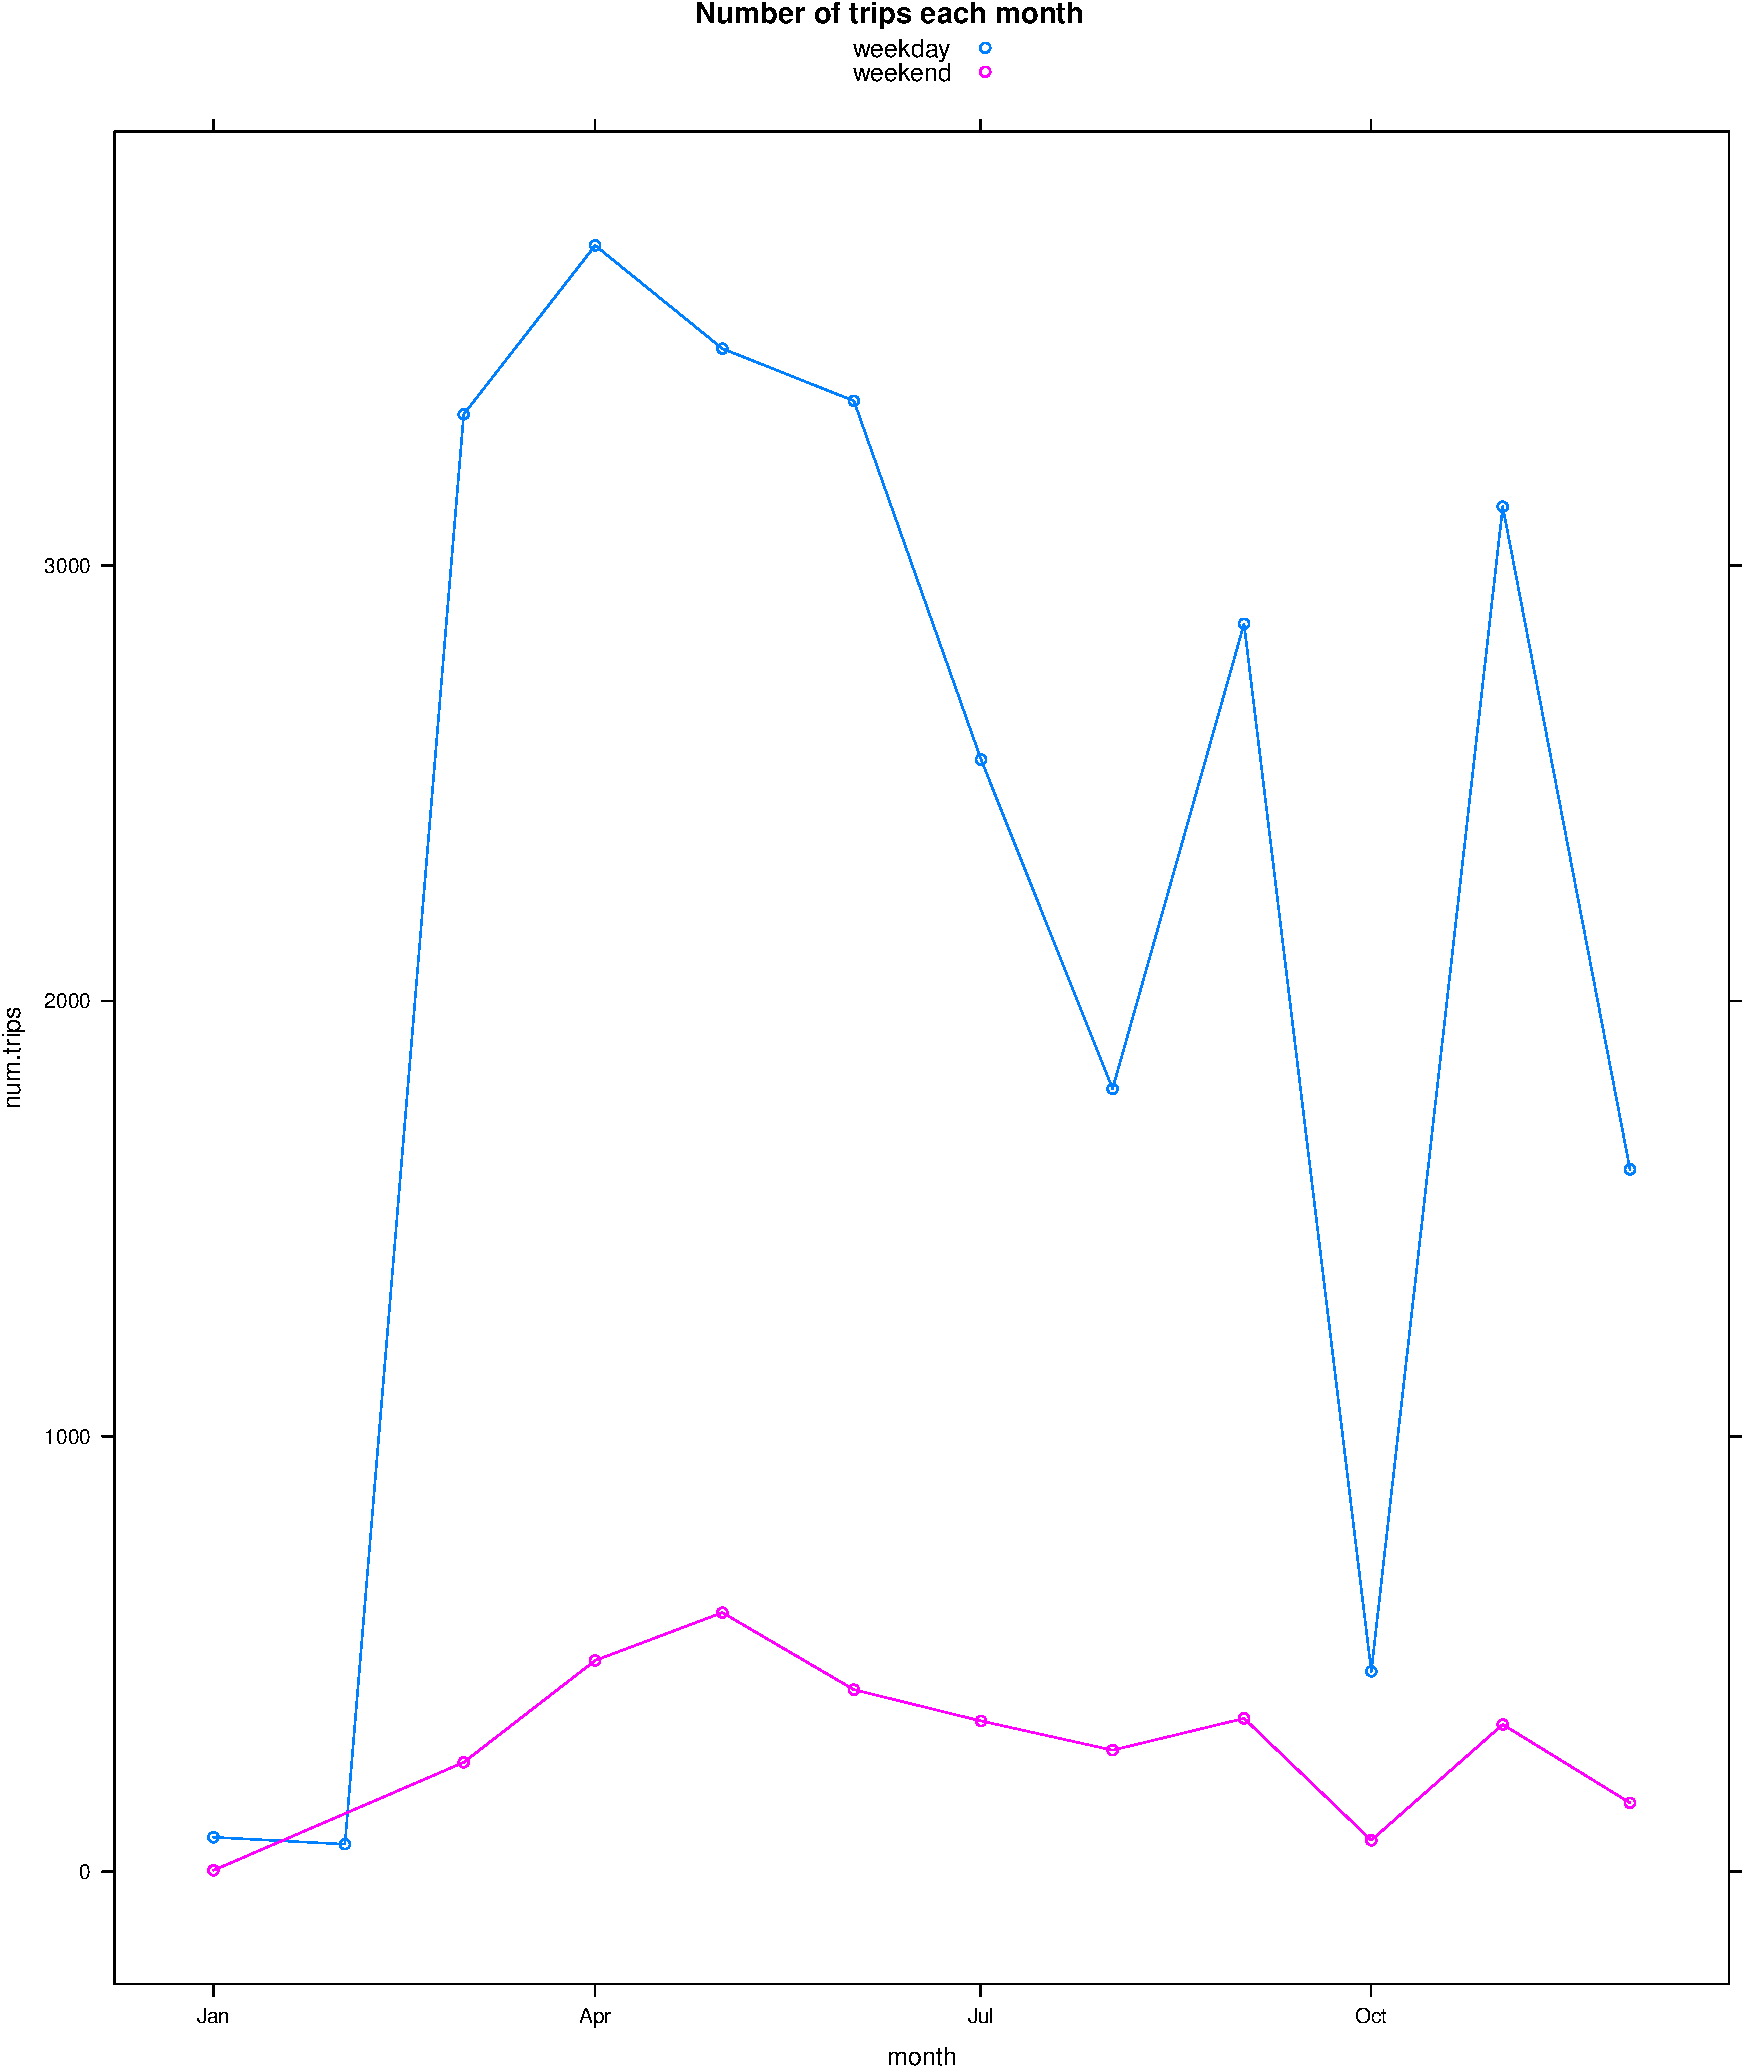
\includegraphics{velopassBirdsEye_files/figure-latex/tripsbymonth-1.pdf}
\caption{}
\end{figure}

We see significant variation in usage over the months, but there may be
a pattern of weekly usage independent of the month. One pattern is that
the usage on weekdays is much larger than that on weekends. The usage
for individual days is hidden under noise, which we can handle by
summing up all days in a month.

\begin{figure}[htbp]
\centering
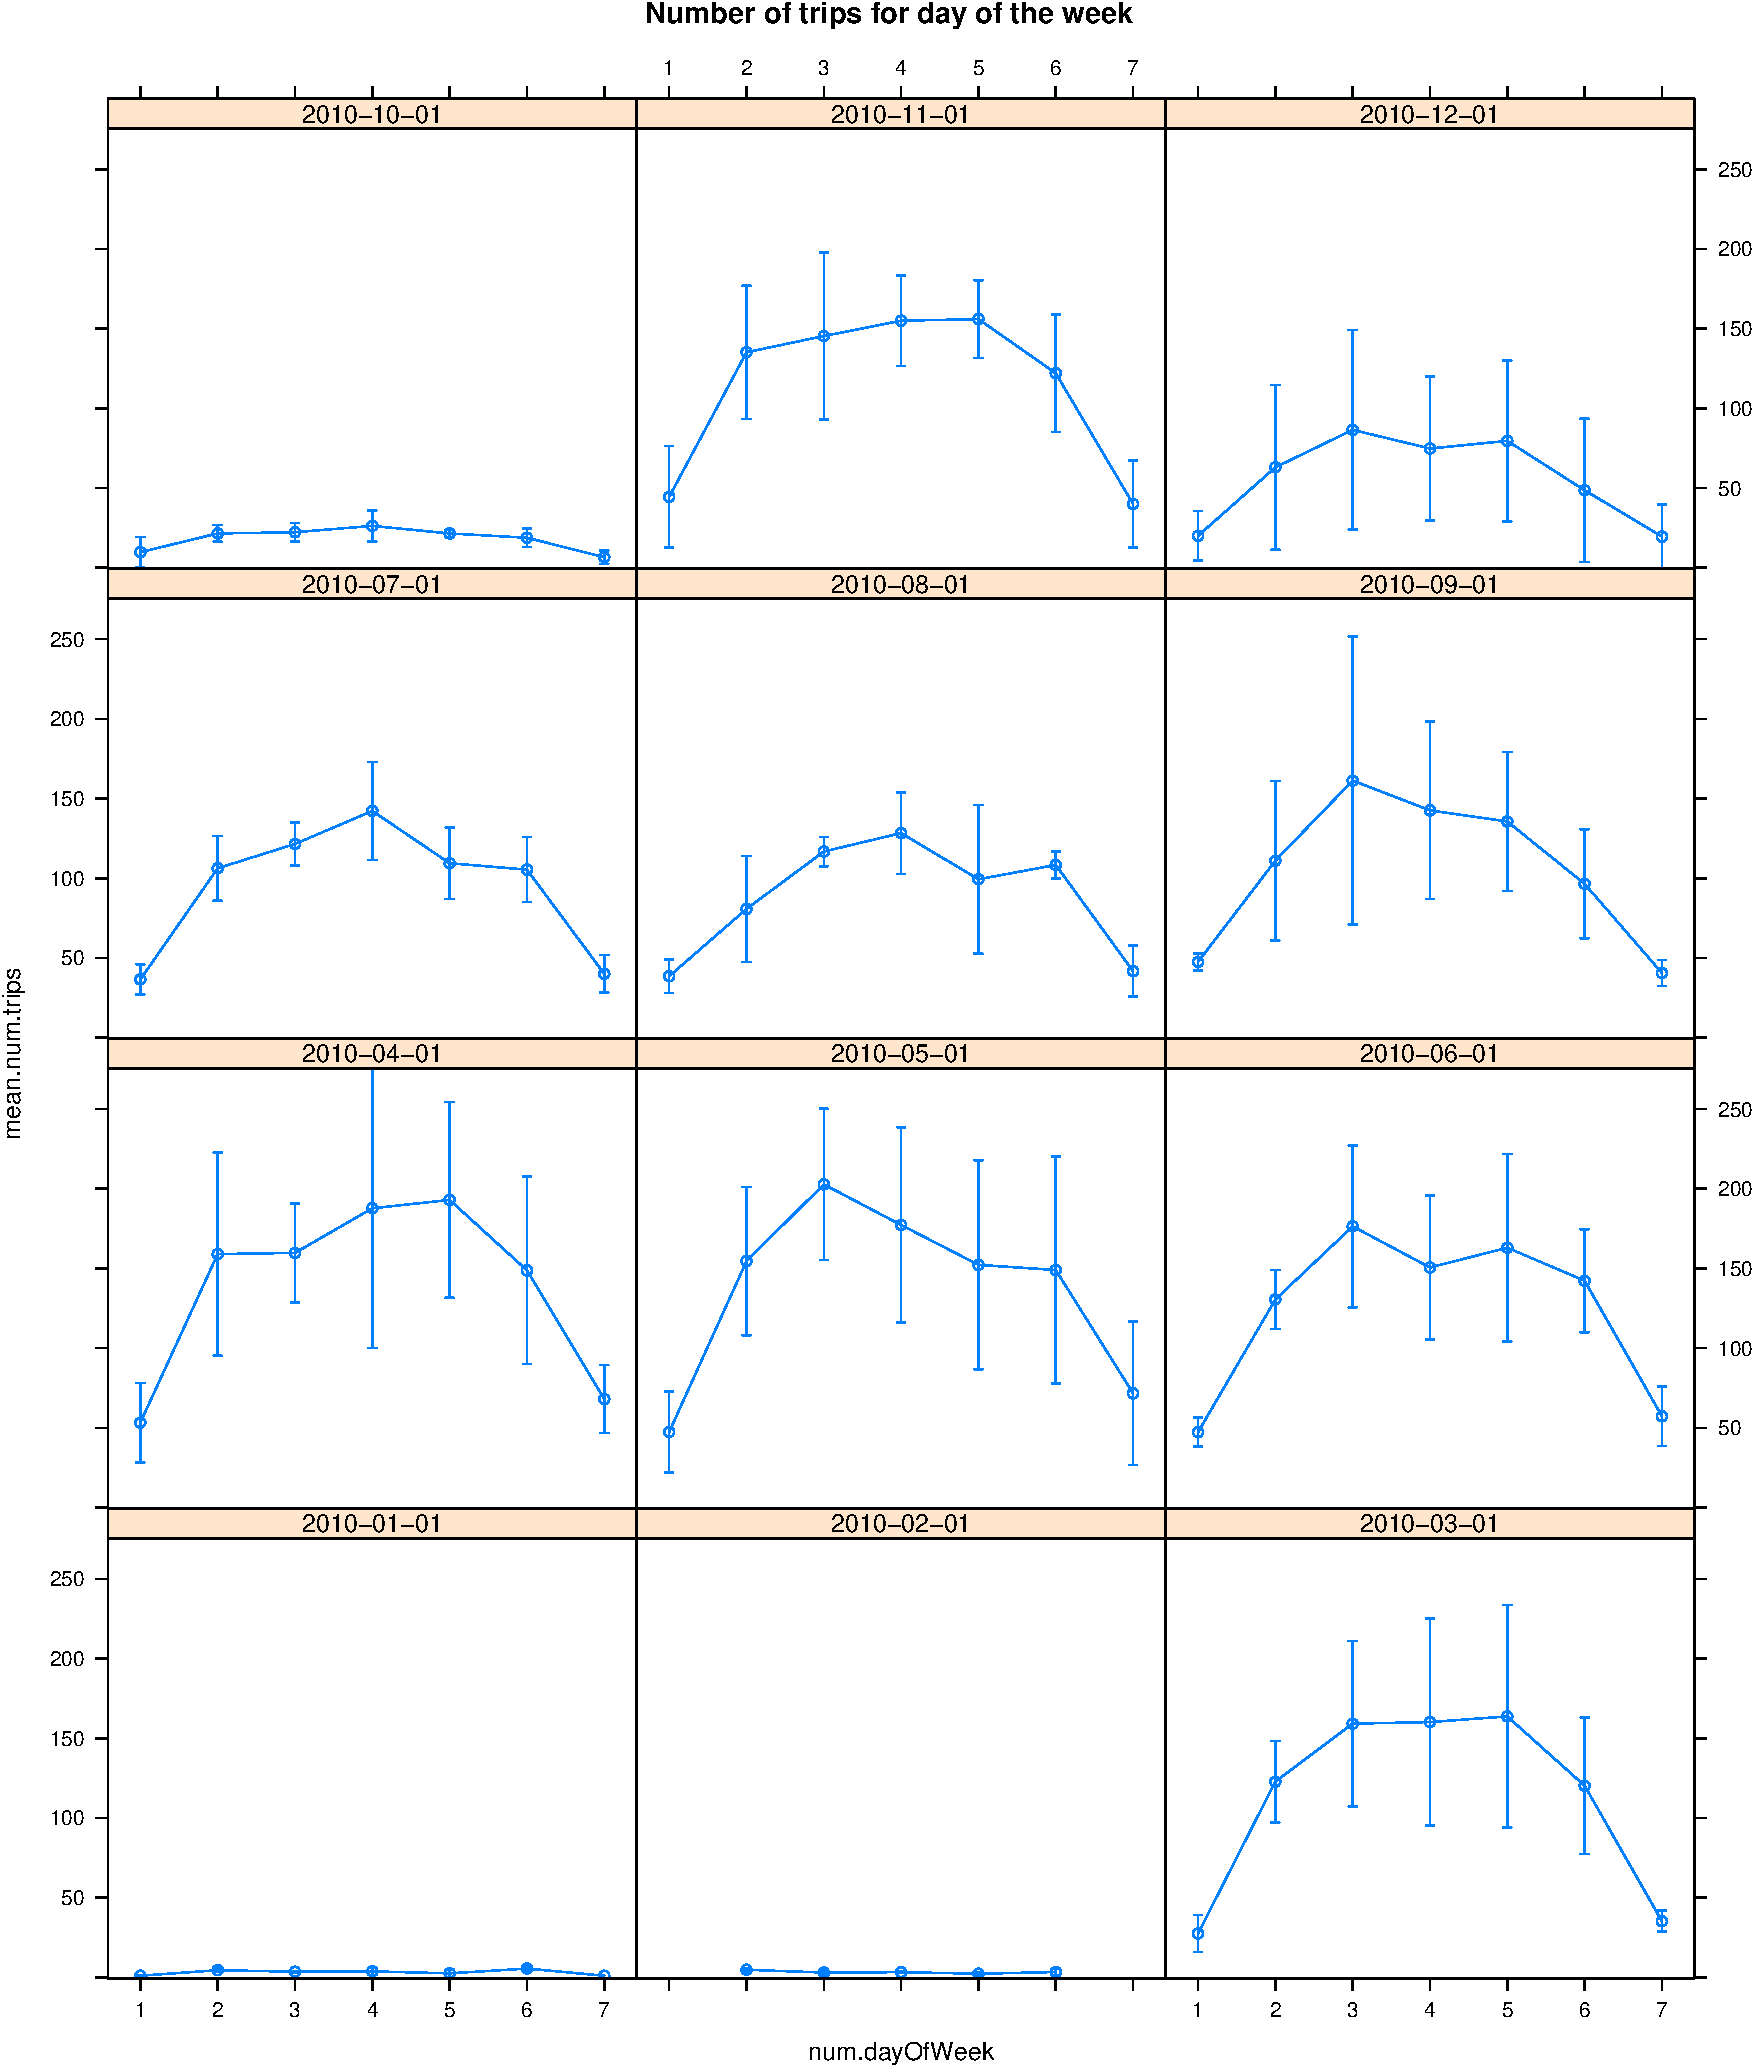
\includegraphics{velopassBirdsEye_files/figure-latex/tripsbydayaggregatemonth-1.pdf}
\caption{}
\end{figure}

We have assumed a normal distribution for the number of trips during a
day to plot the error bars as the standard deviation from the mean.
However we should expect number of trips in a day to be Poisson
distributed.

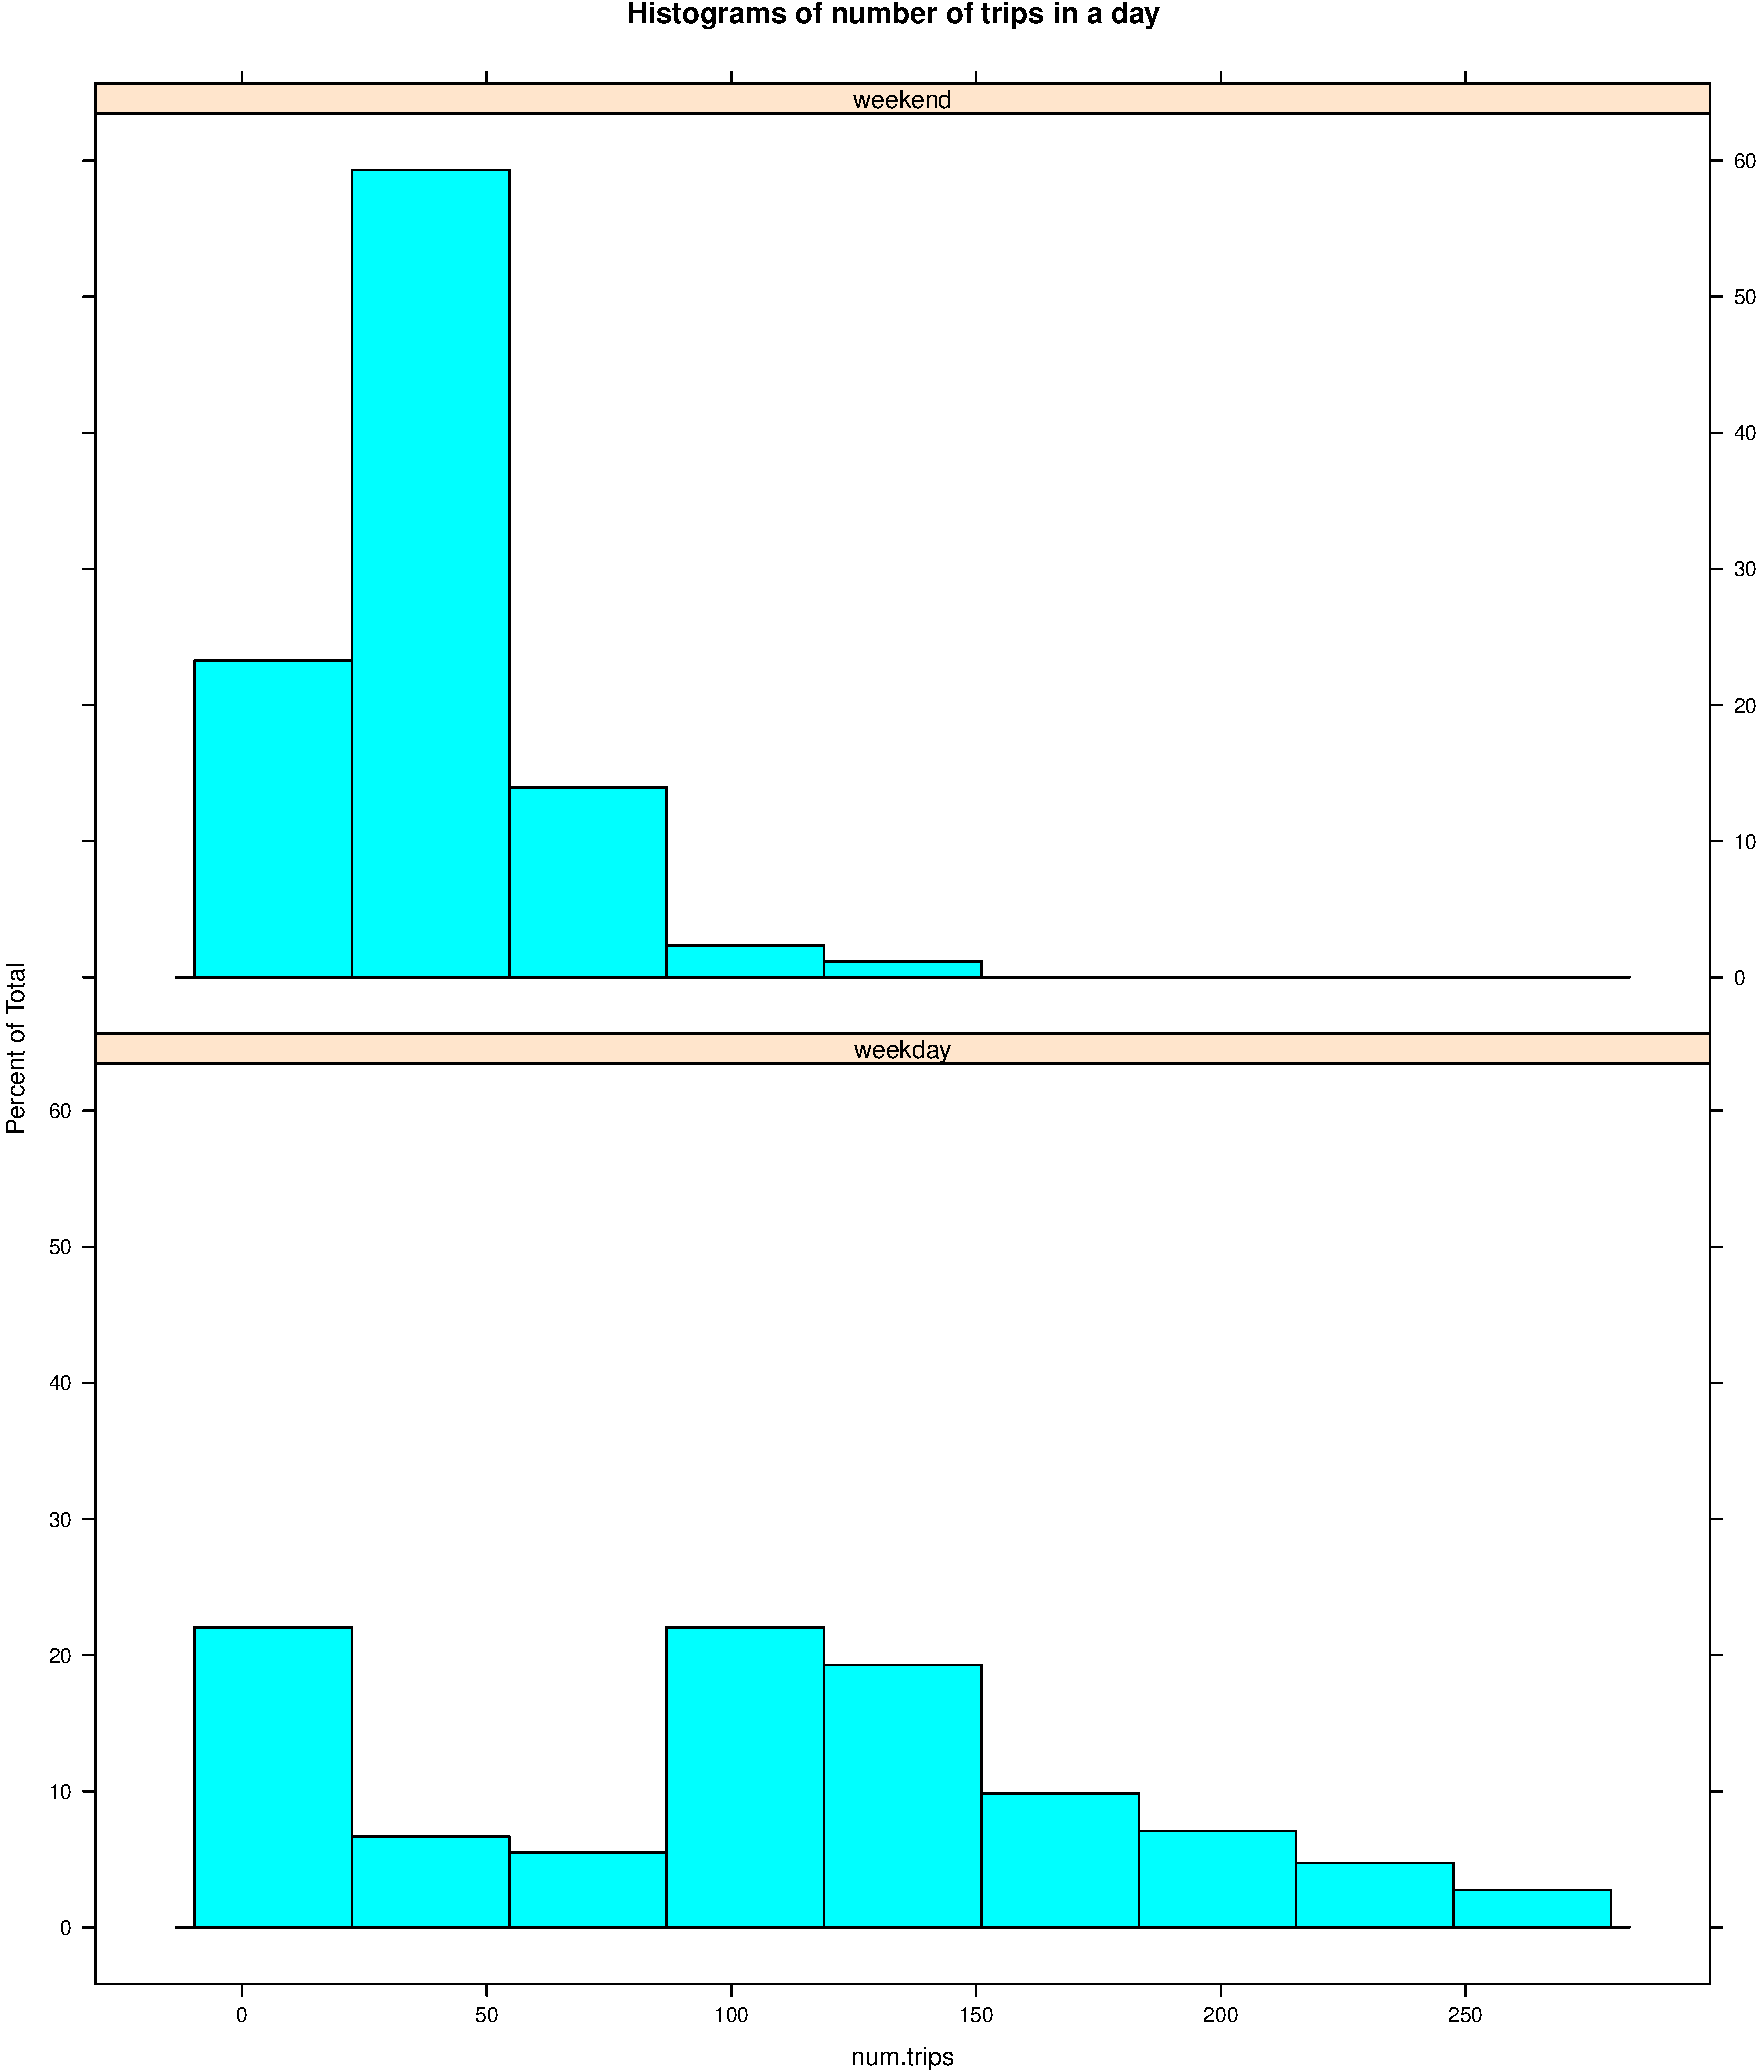
\includegraphics{velopassBirdsEye_files/figure-latex/histtripsdistbn-1.pdf}
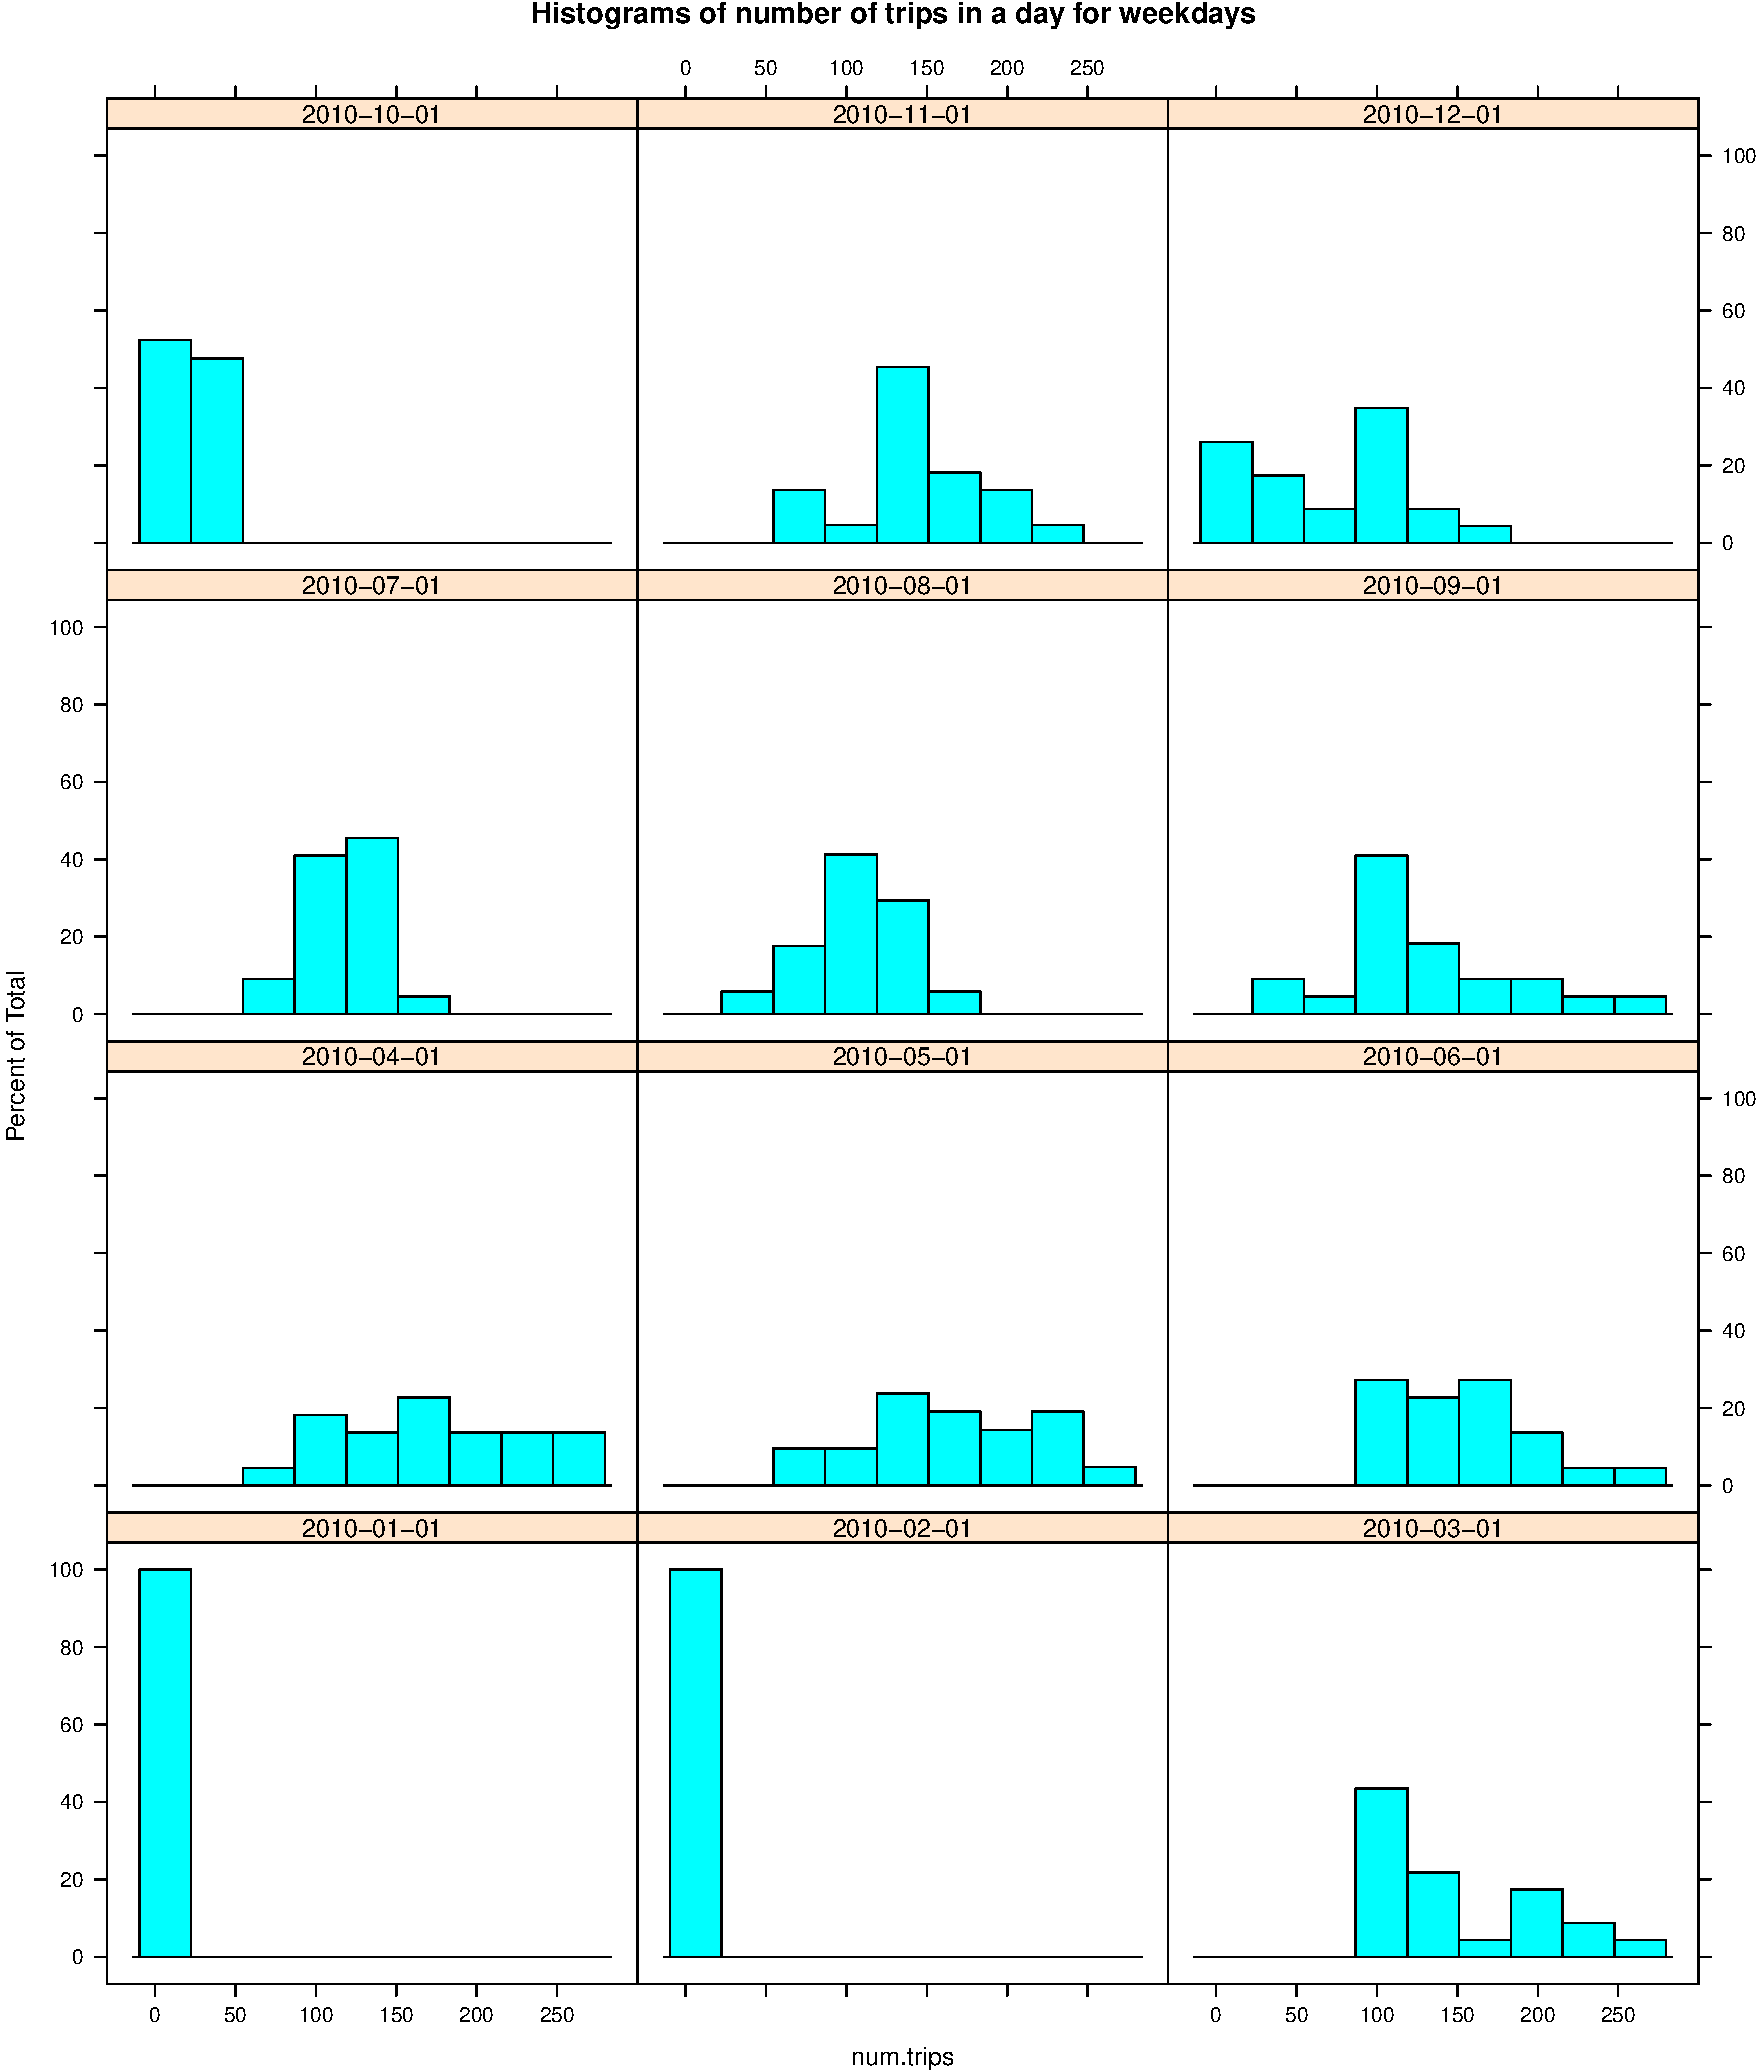
\includegraphics{velopassBirdsEye_files/figure-latex/histtripsdistbn-2.pdf}
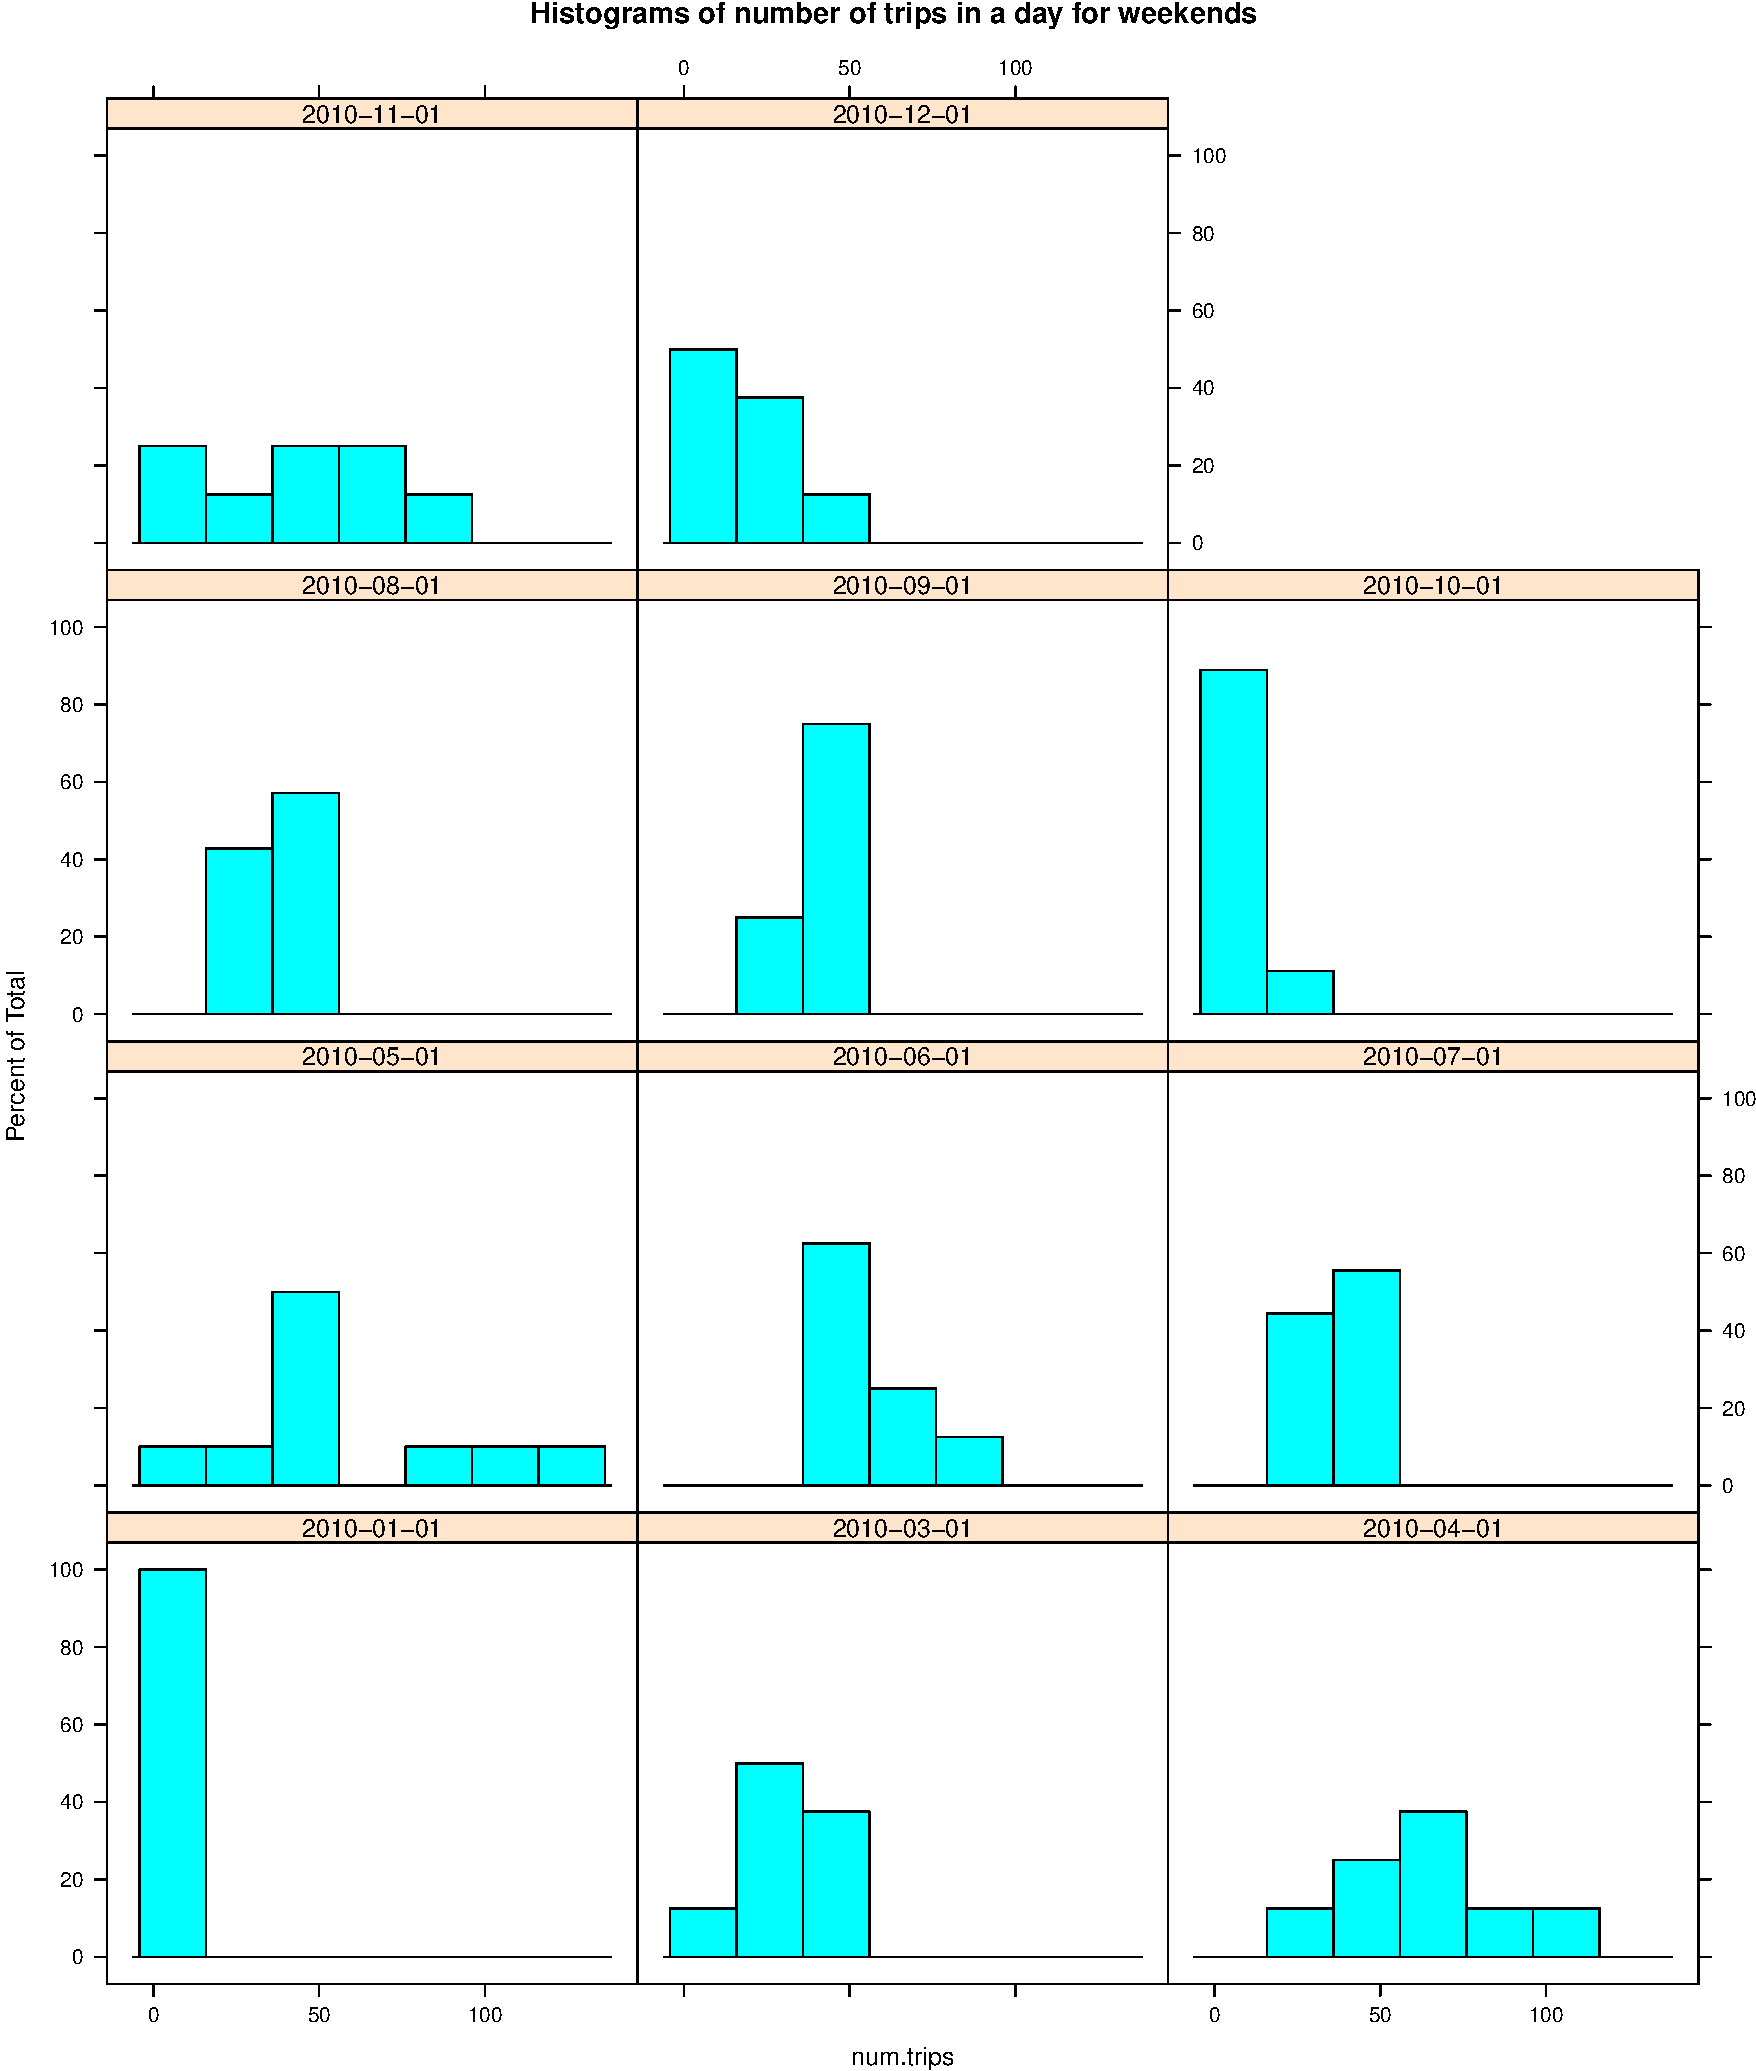
\includegraphics{velopassBirdsEye_files/figure-latex/histtripsdistbn-3.pdf}

We can look for number of trips during certain hours of the day,
summed/averaged over days/weeks/months/years. We first need a function
that converts time of day to seconds.

We can use the functions to count trips to find trips by the hour. First
we write a function that will get the counts for every hour of the day,
and include an offset in minutes.

Now we can make some plots for usage by the hour over the entire time
duration of the data.

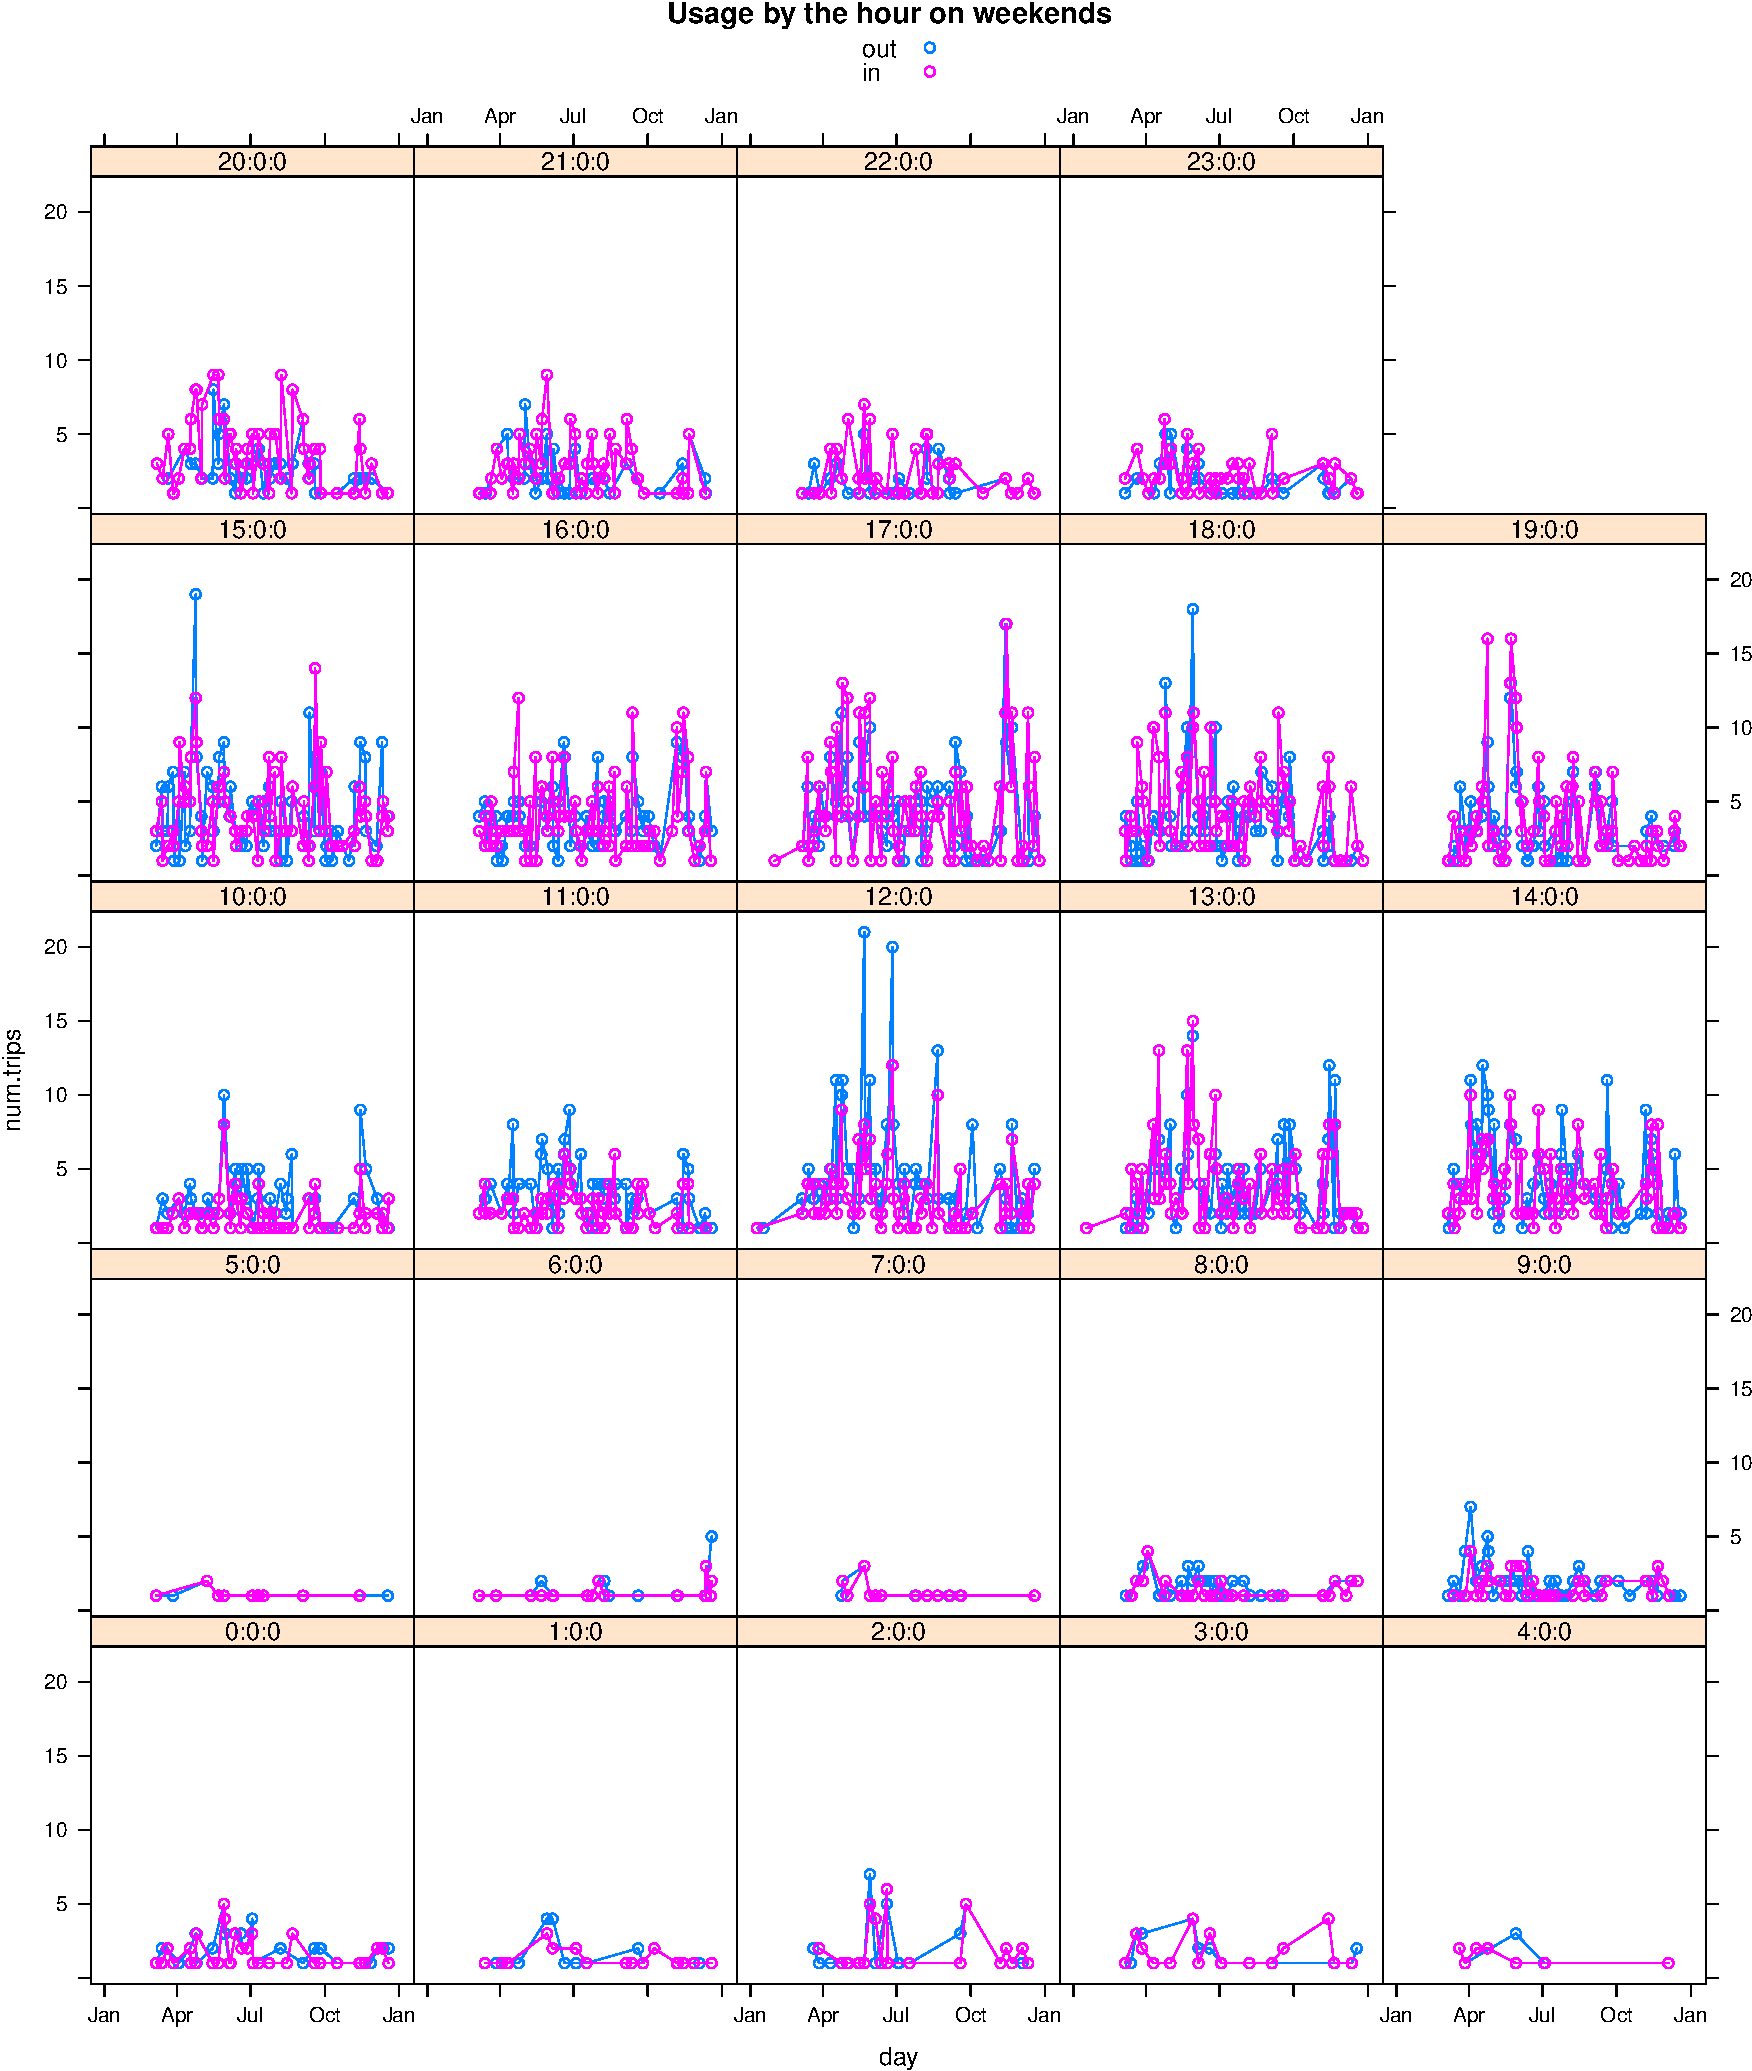
\includegraphics{velopassBirdsEye_files/figure-latex/dailyusagebythehour-1.pdf}
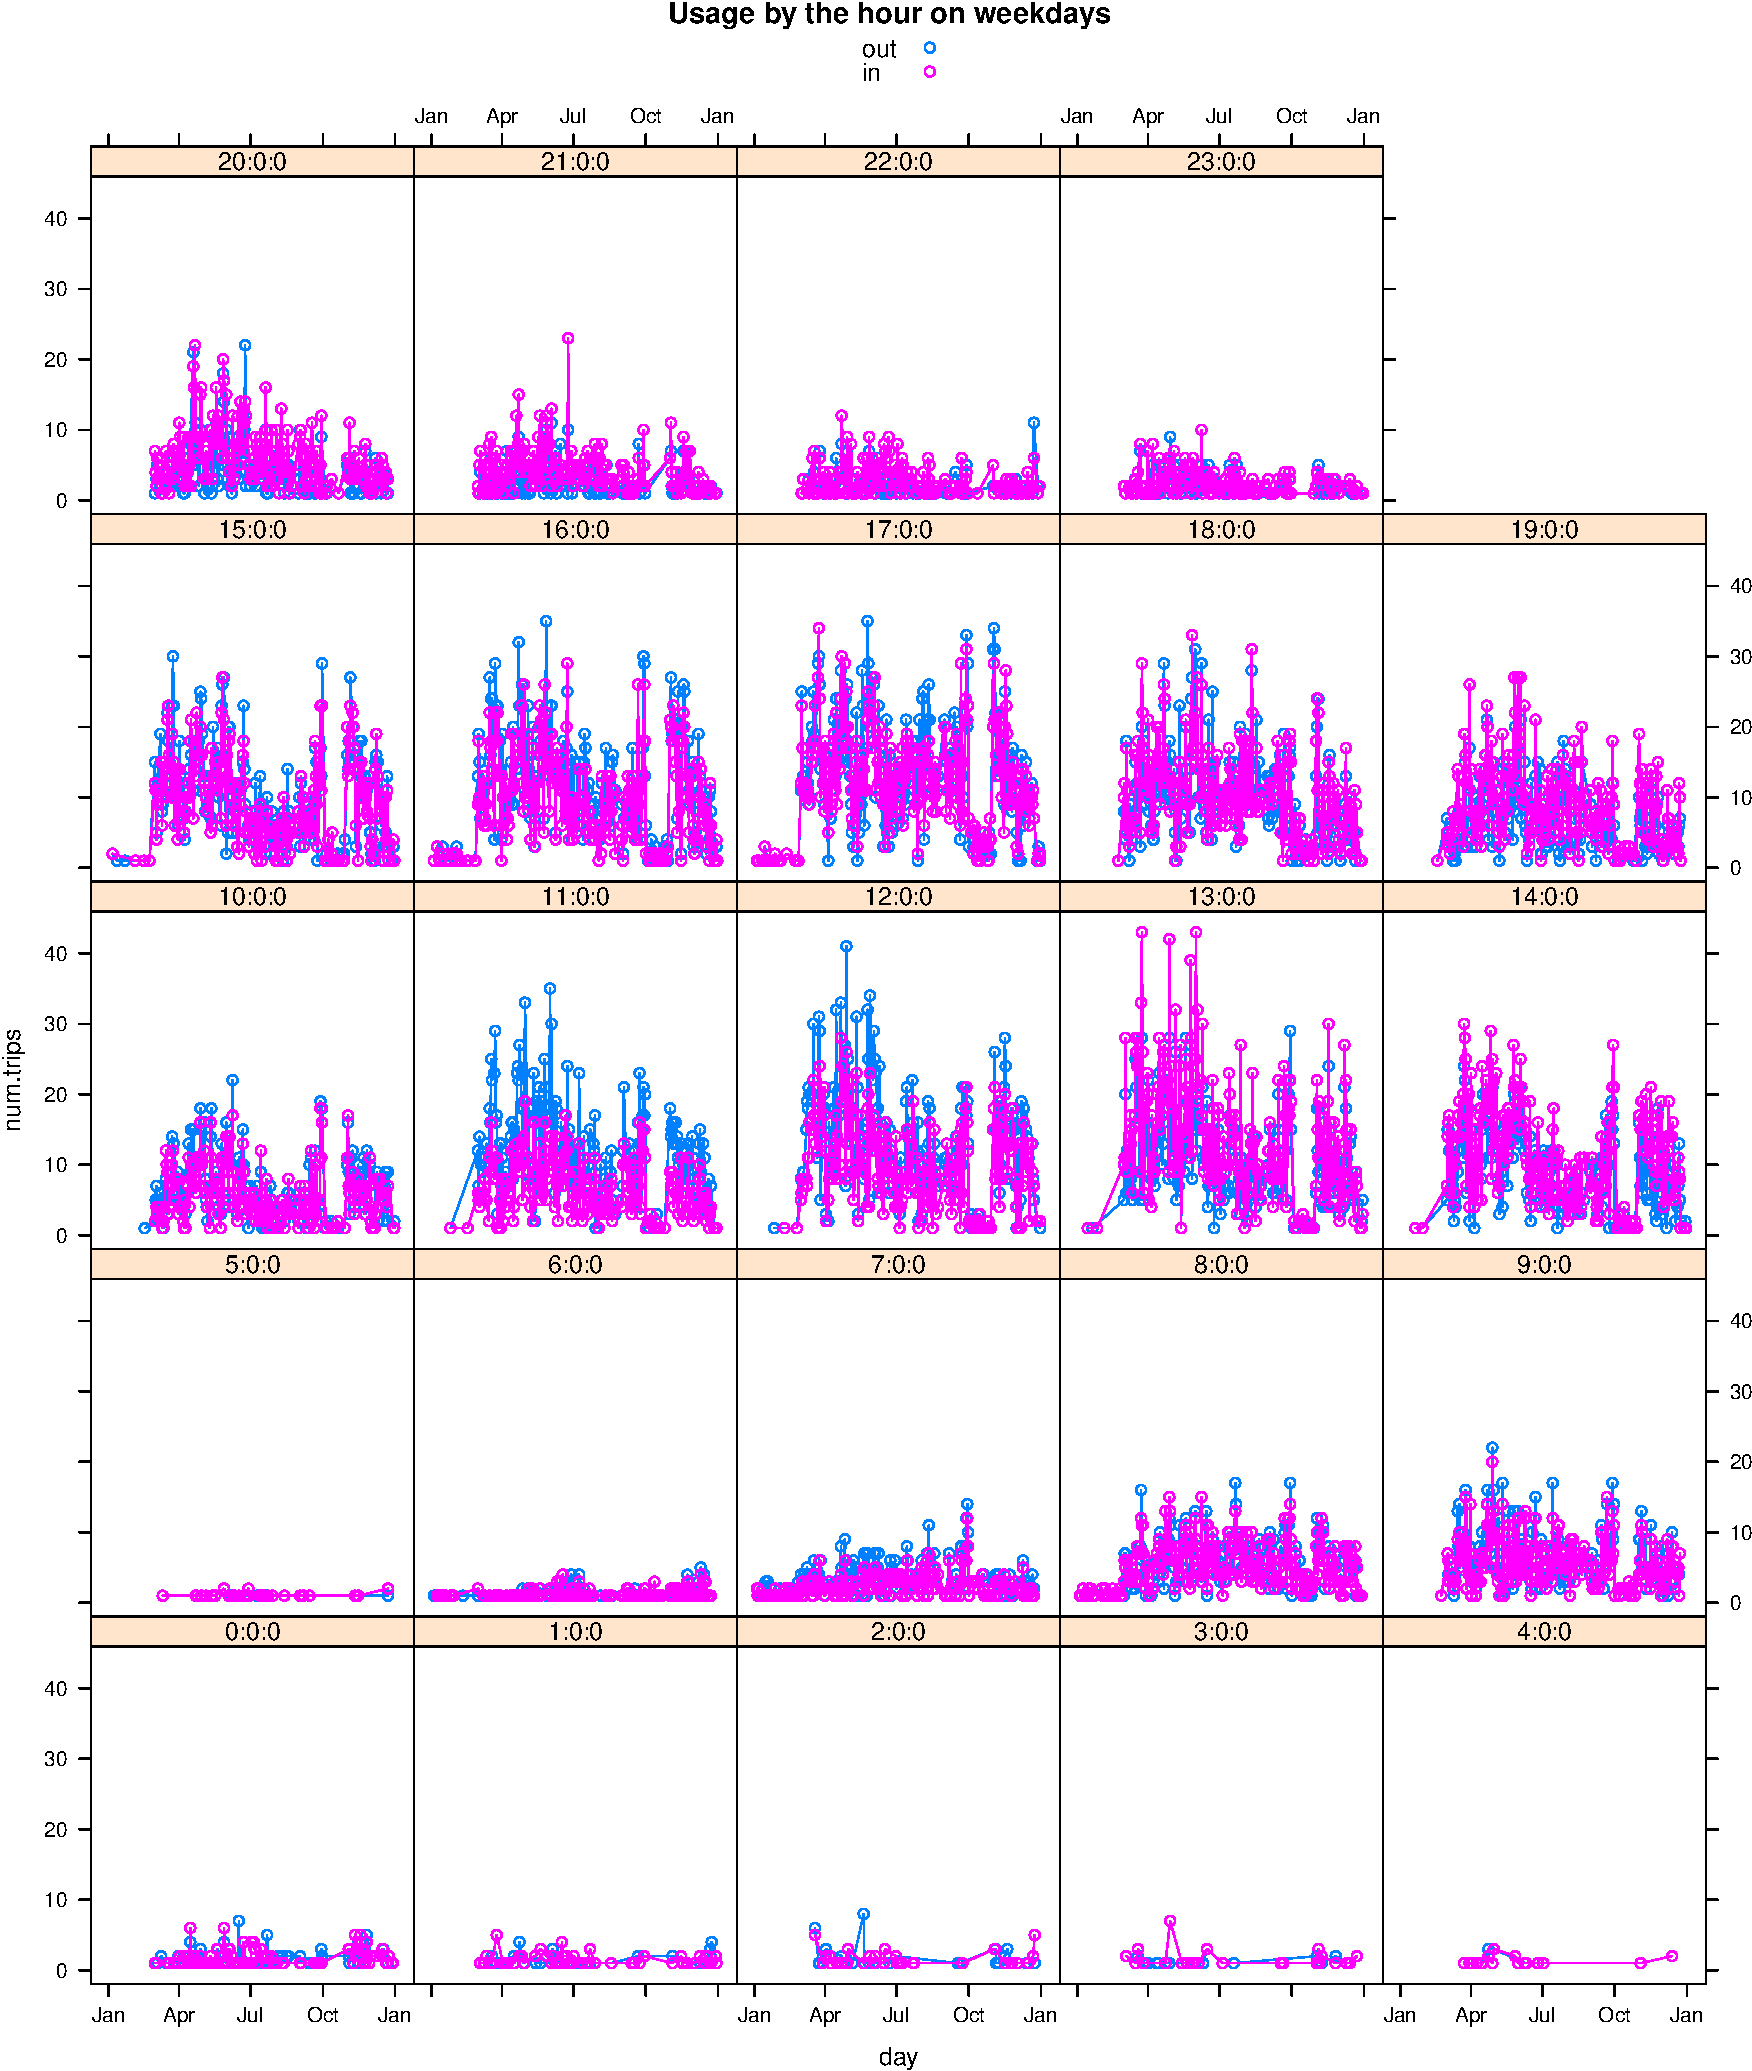
\includegraphics{velopassBirdsEye_files/figure-latex/dailyusagebythehour-2.pdf}

So far we have looked at the behavior of number of trips in a day. What
we would also want to see how many trips are made over a certain period
of the day. We can use the data produced by \emph{countTripsHourly} to
make these plots as well,

\begin{figure}[htbp]
\centering
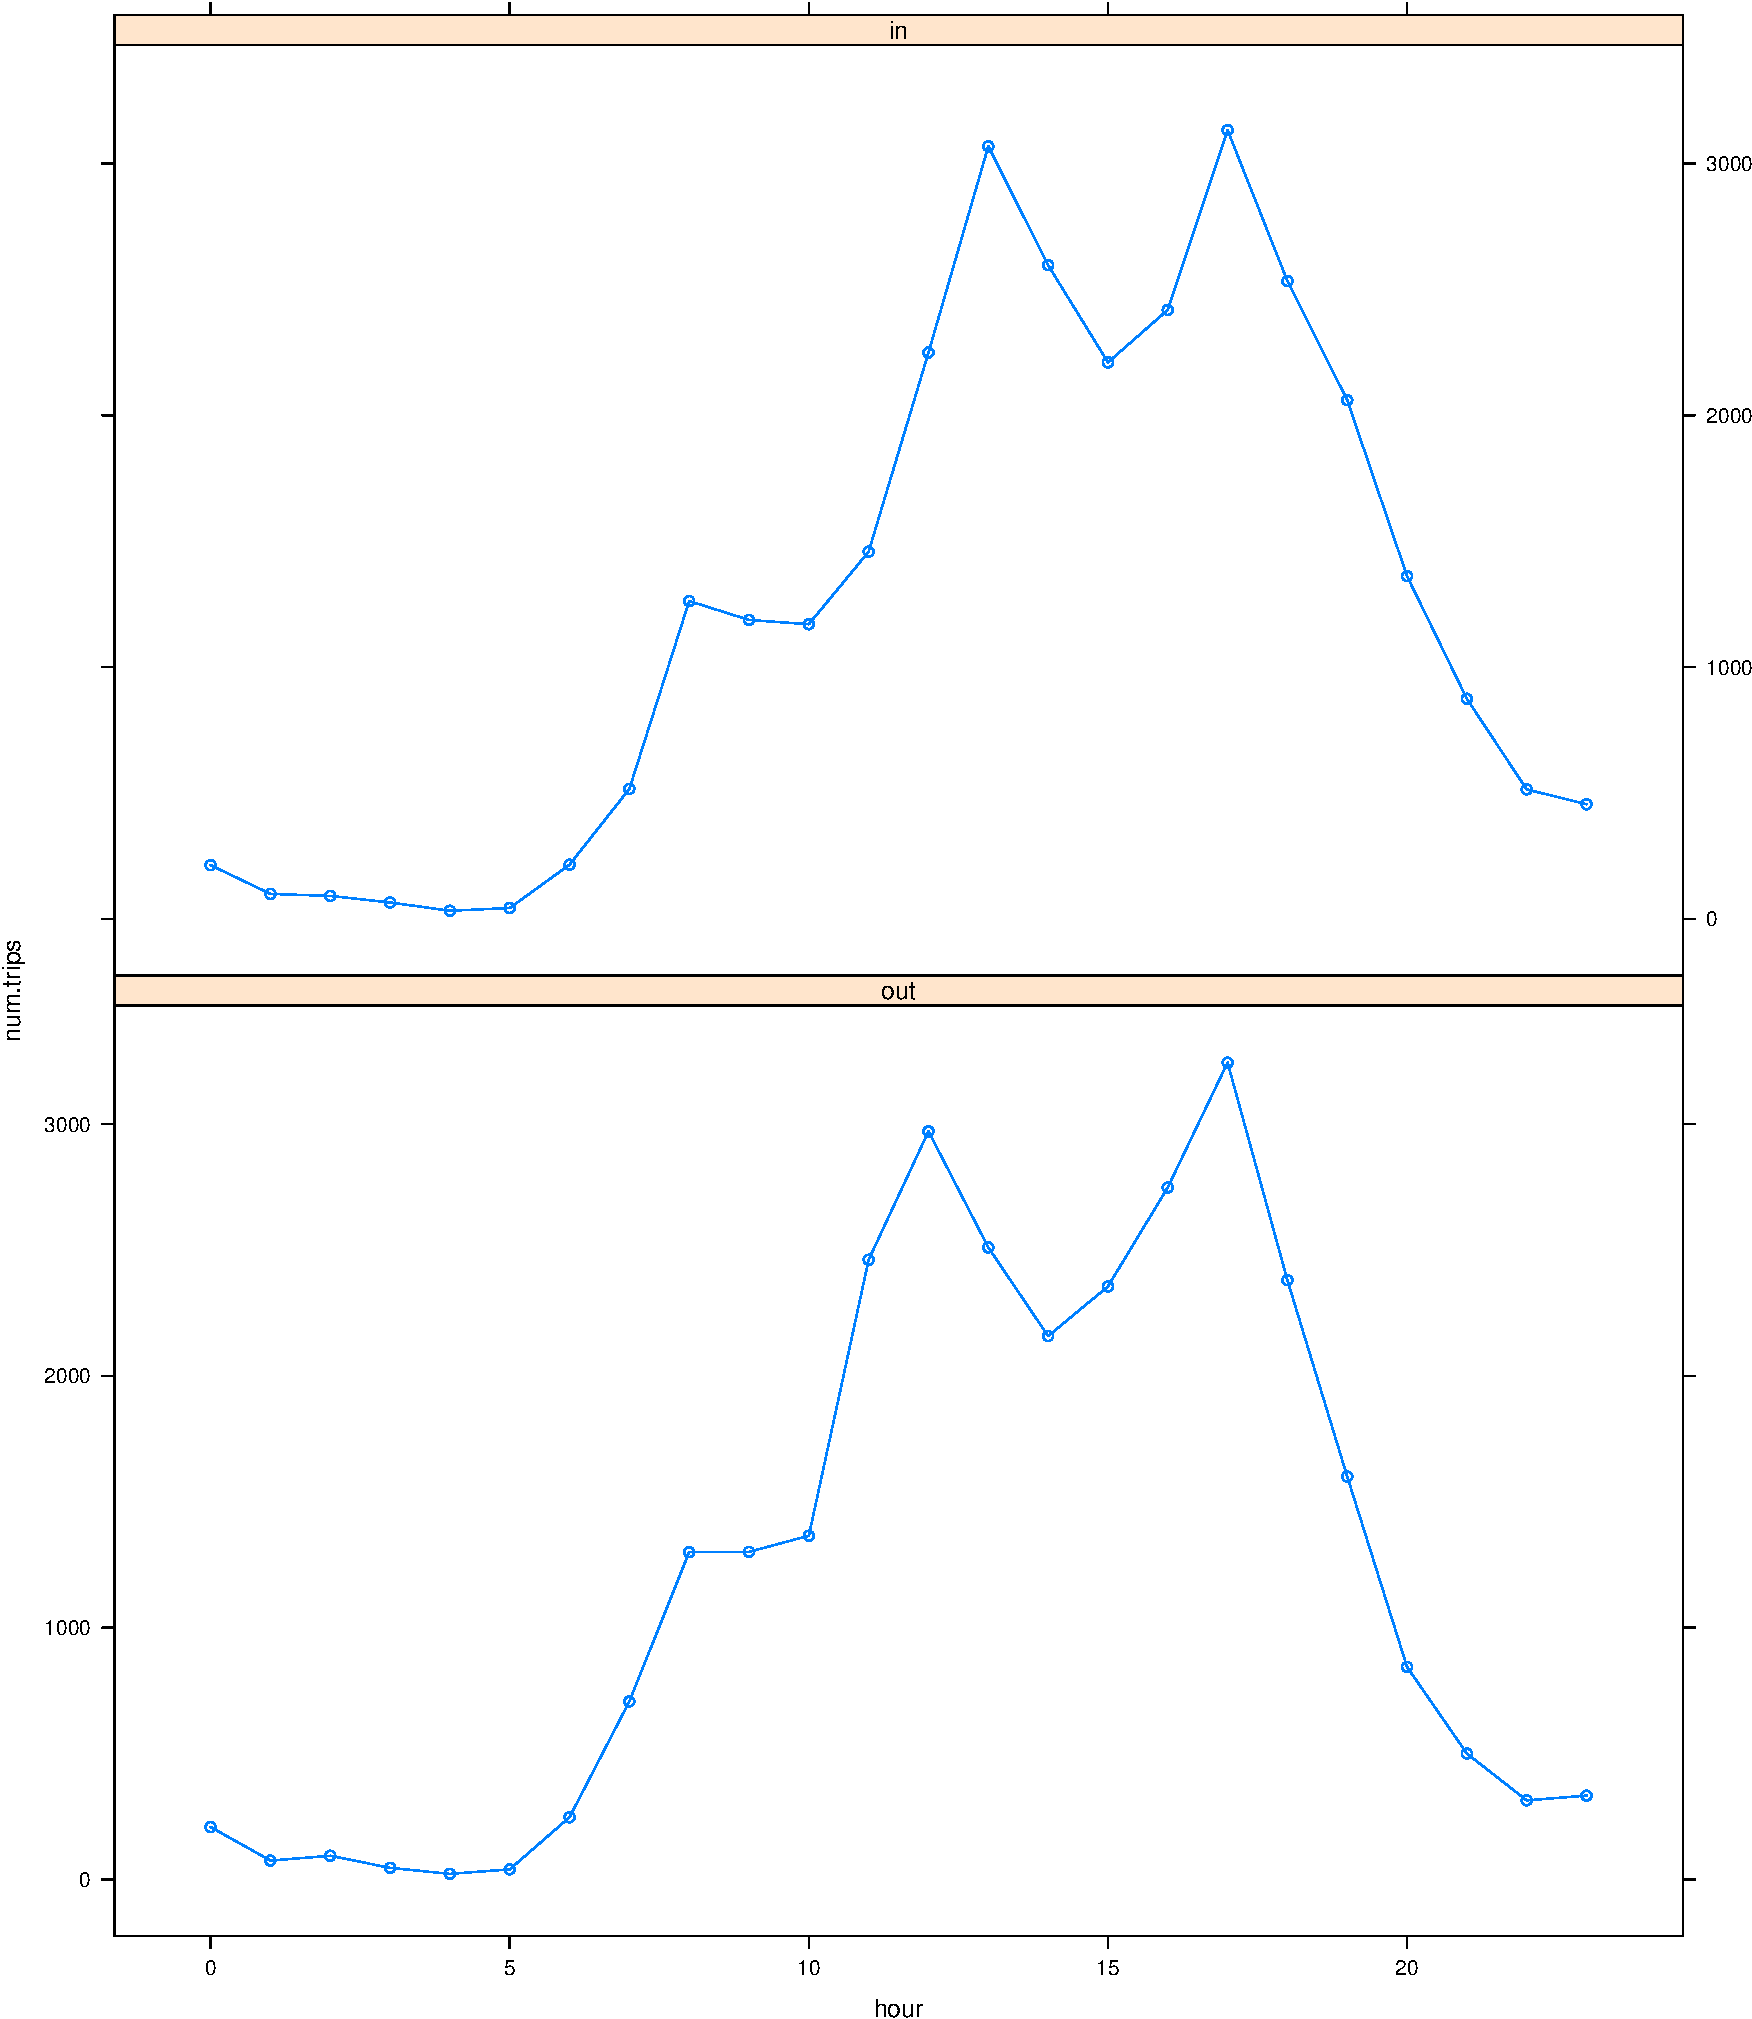
\includegraphics{velopassBirdsEye_files/figure-latex/hourlyusage-1.pdf}
\caption{}
\end{figure}

Above we saw total hourly usage for the whole year (all the data in
\emph{vlp2010}), and we can aggregate the trips for each month, or for
each week as well.

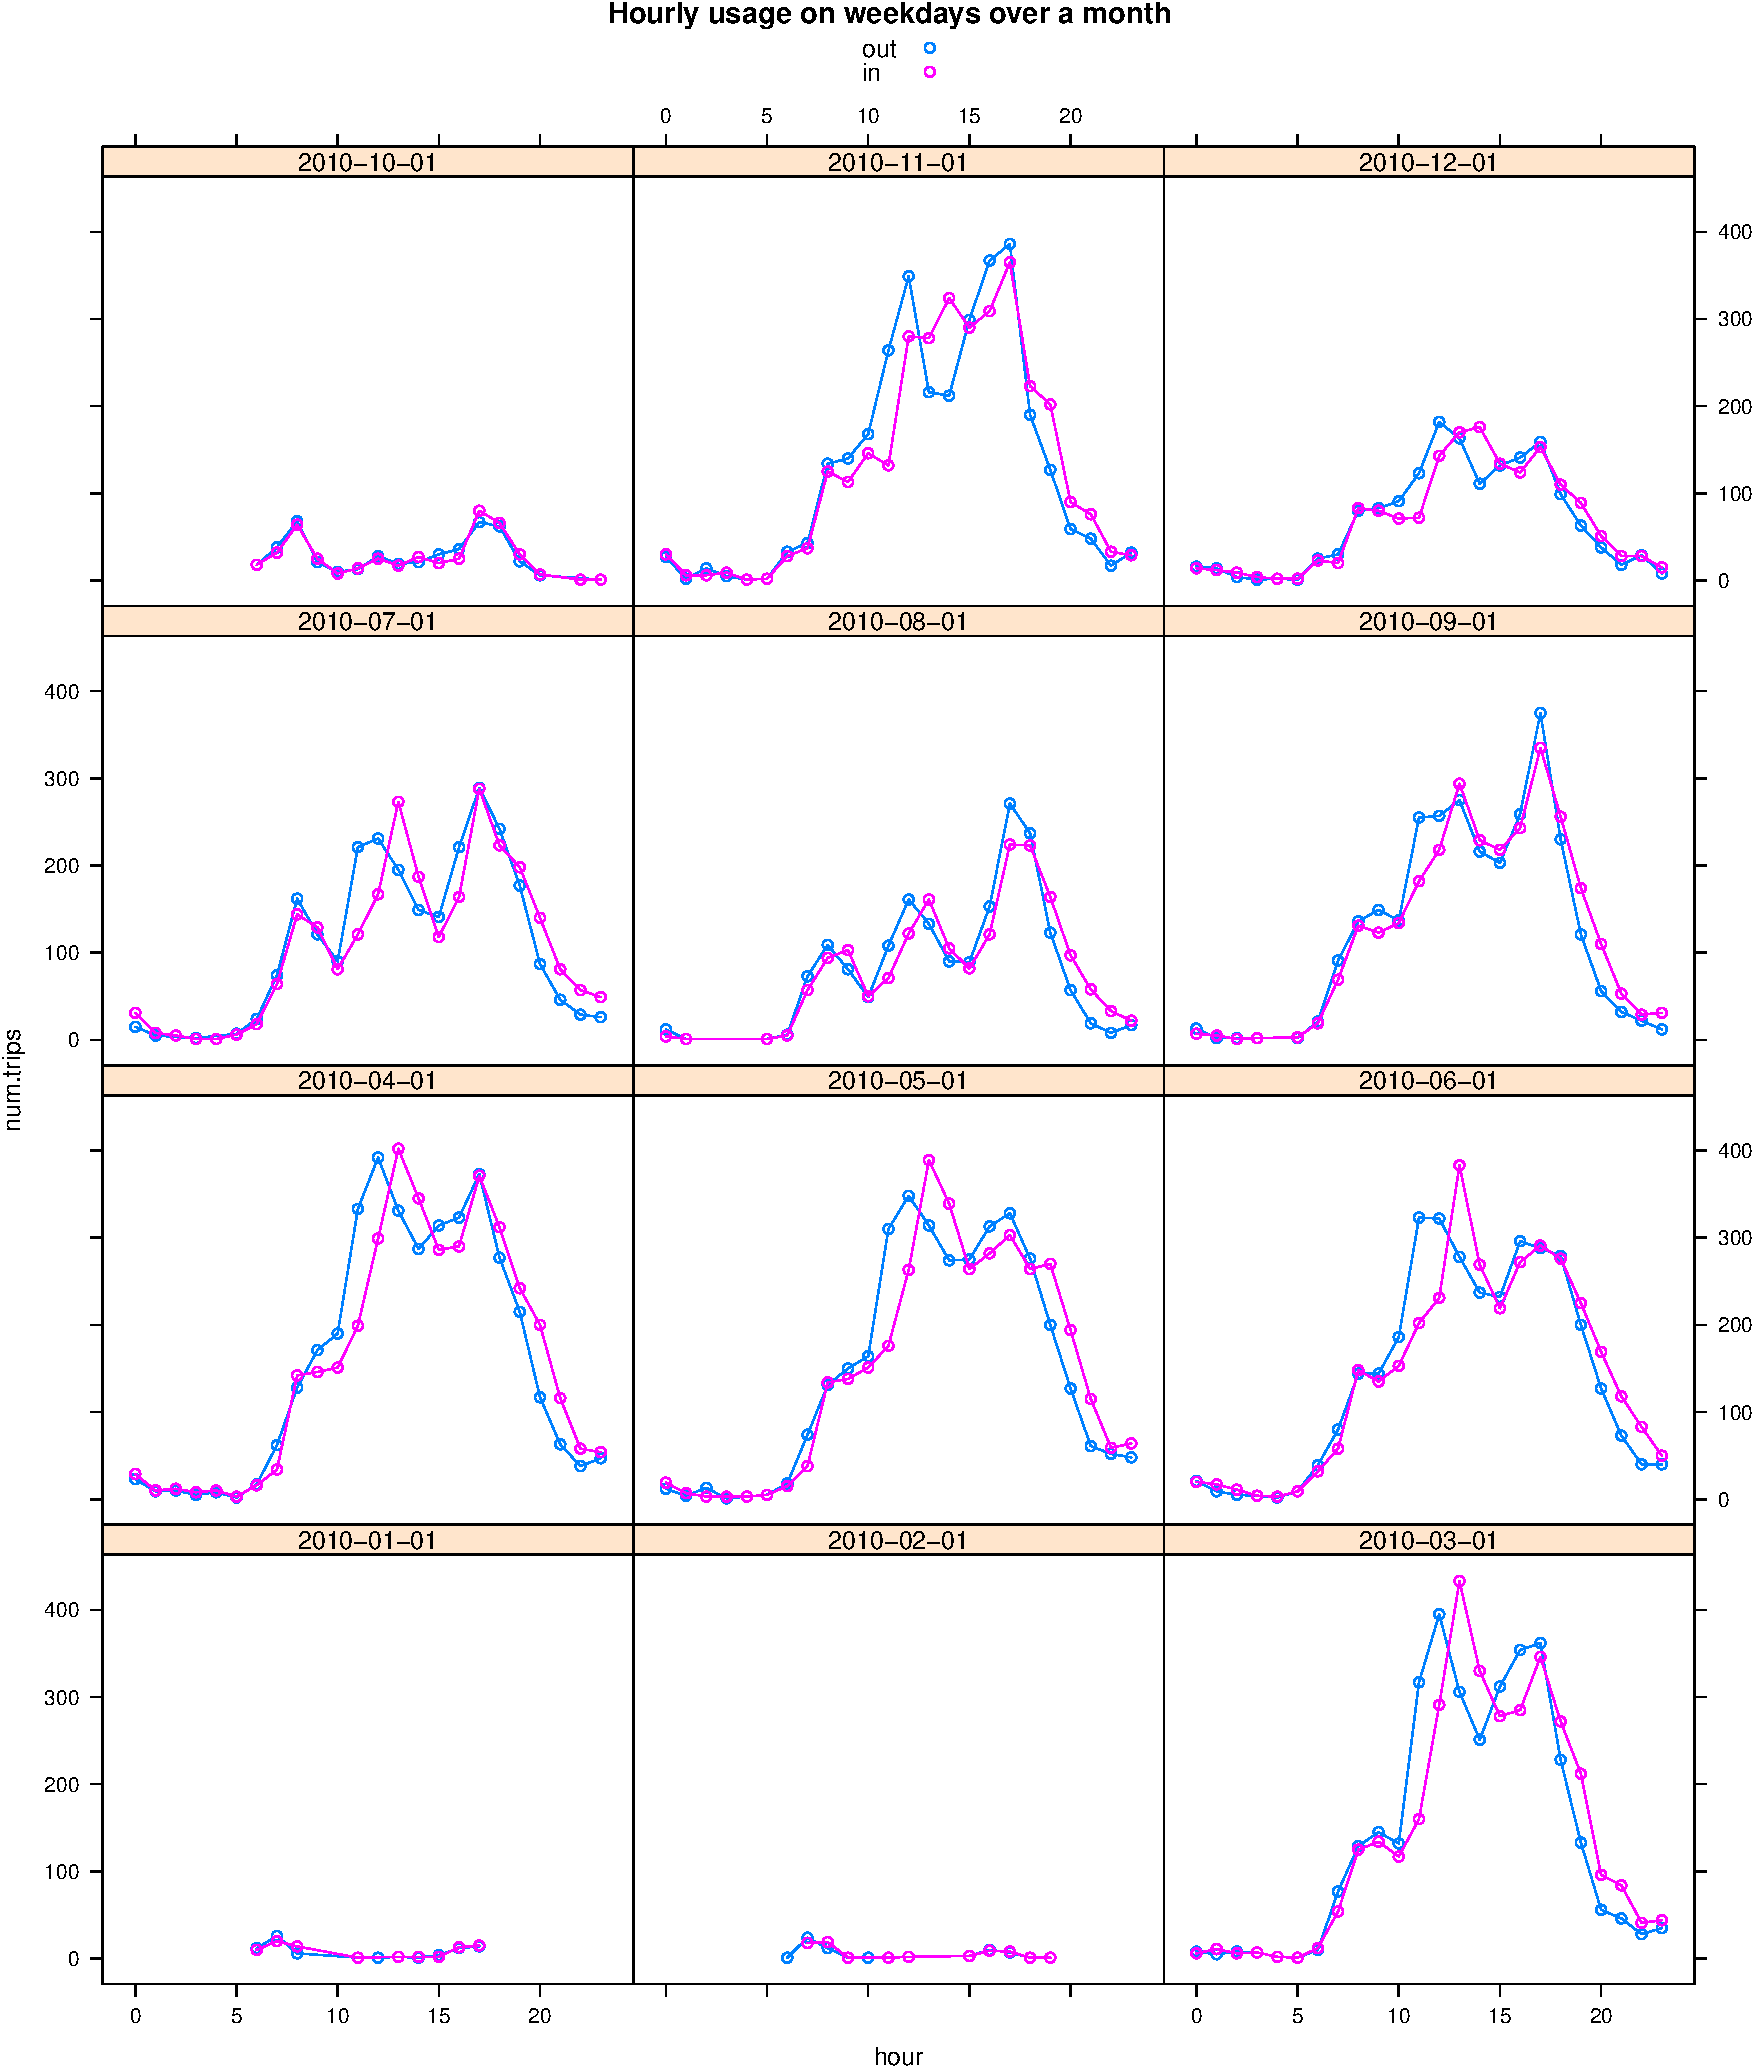
\includegraphics{velopassBirdsEye_files/figure-latex/hourlyusagemonth-1.pdf}
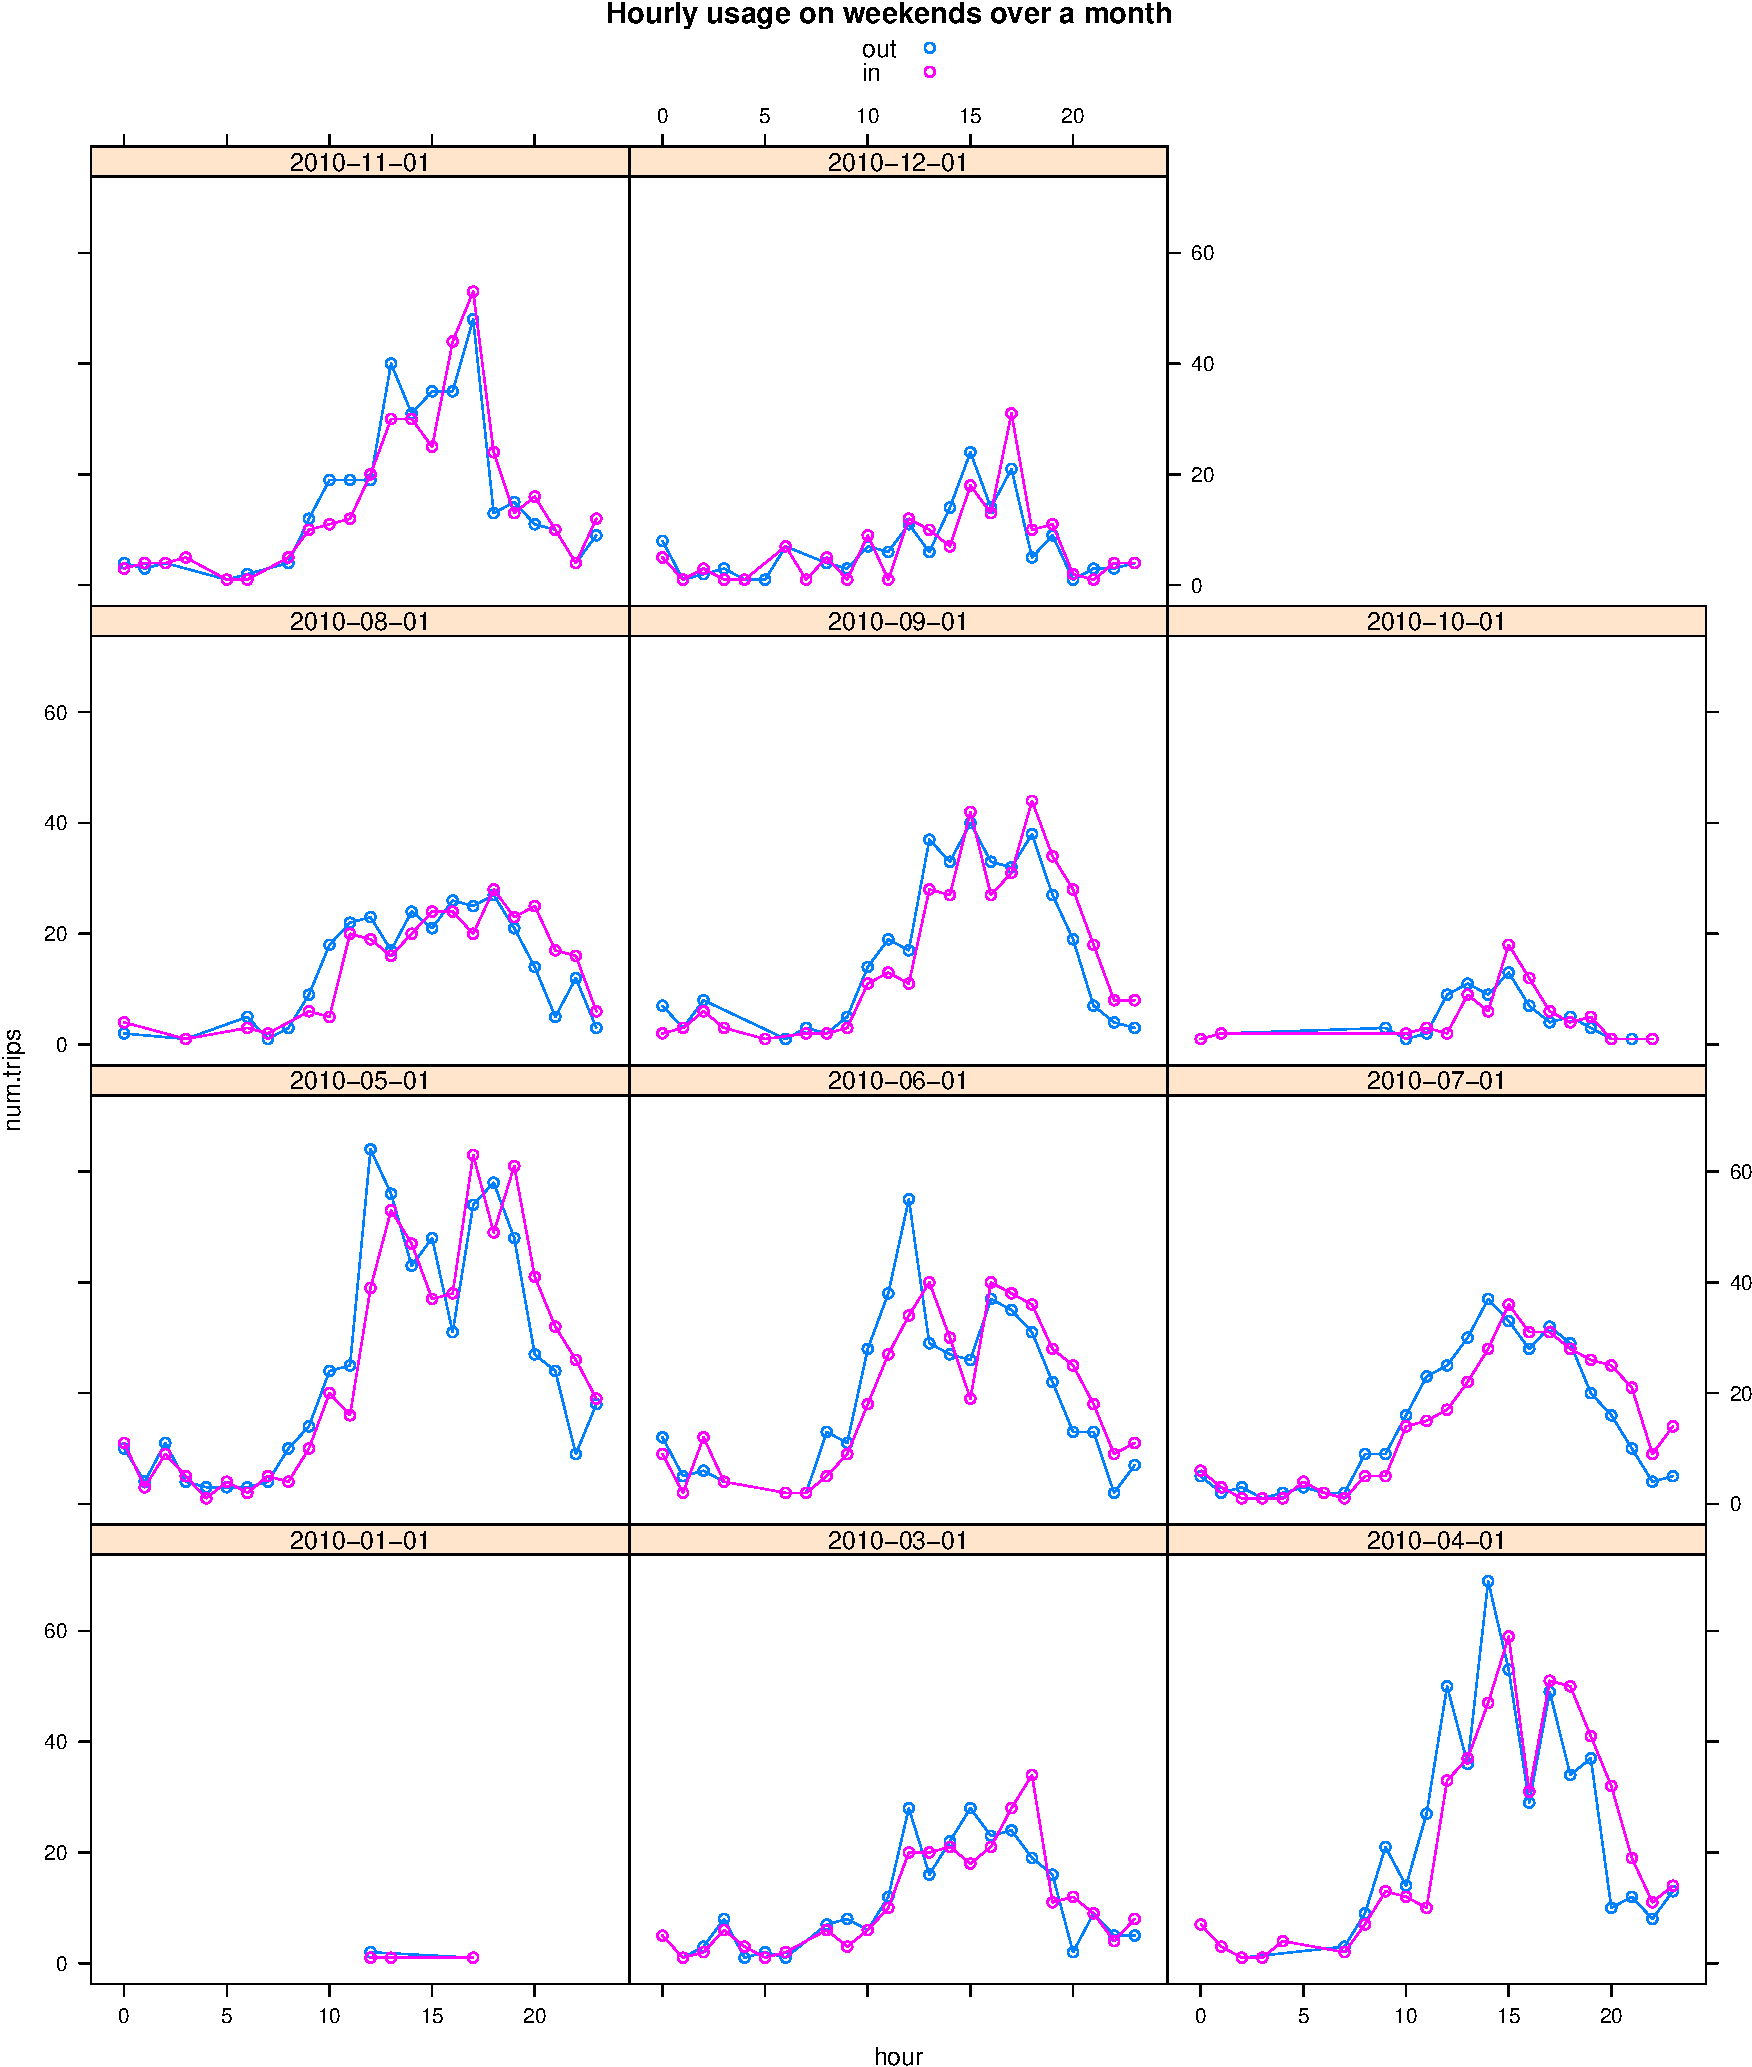
\includegraphics{velopassBirdsEye_files/figure-latex/hourlyusagemonth-2.pdf}

\subsection{Trip durations}\label{trip-durations}

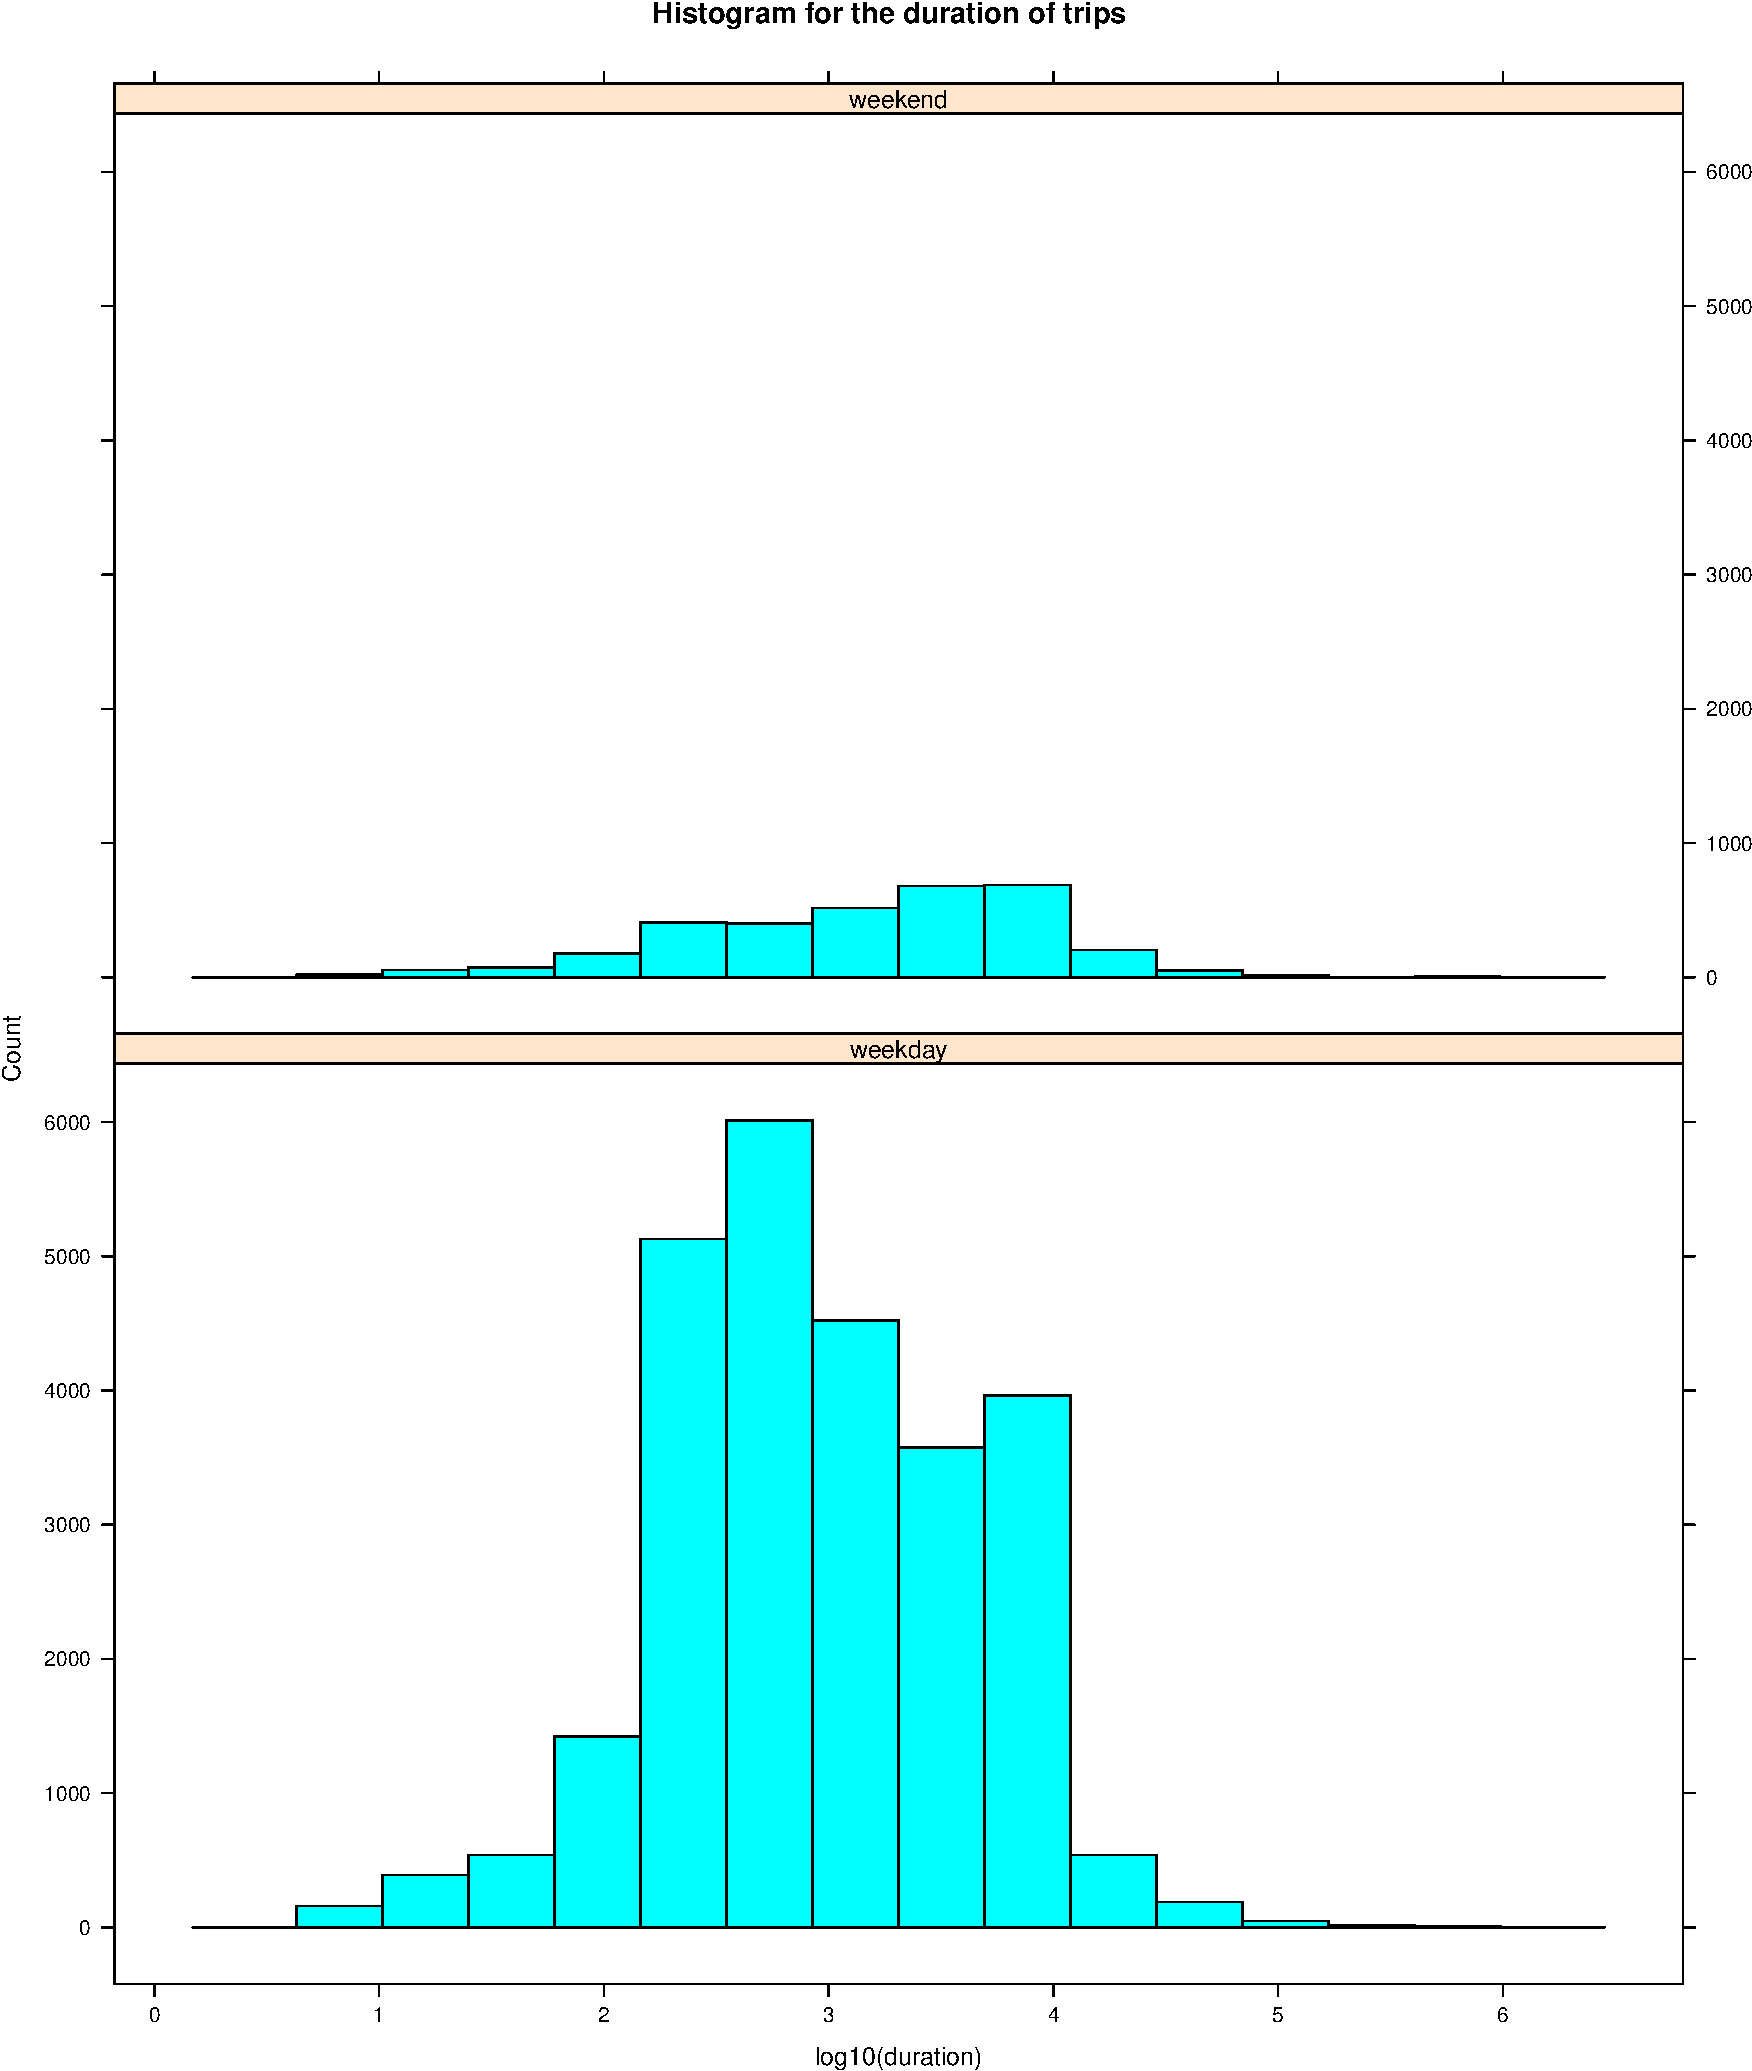
\includegraphics{velopassBirdsEye_files/figure-latex/tripdurations-1.pdf}
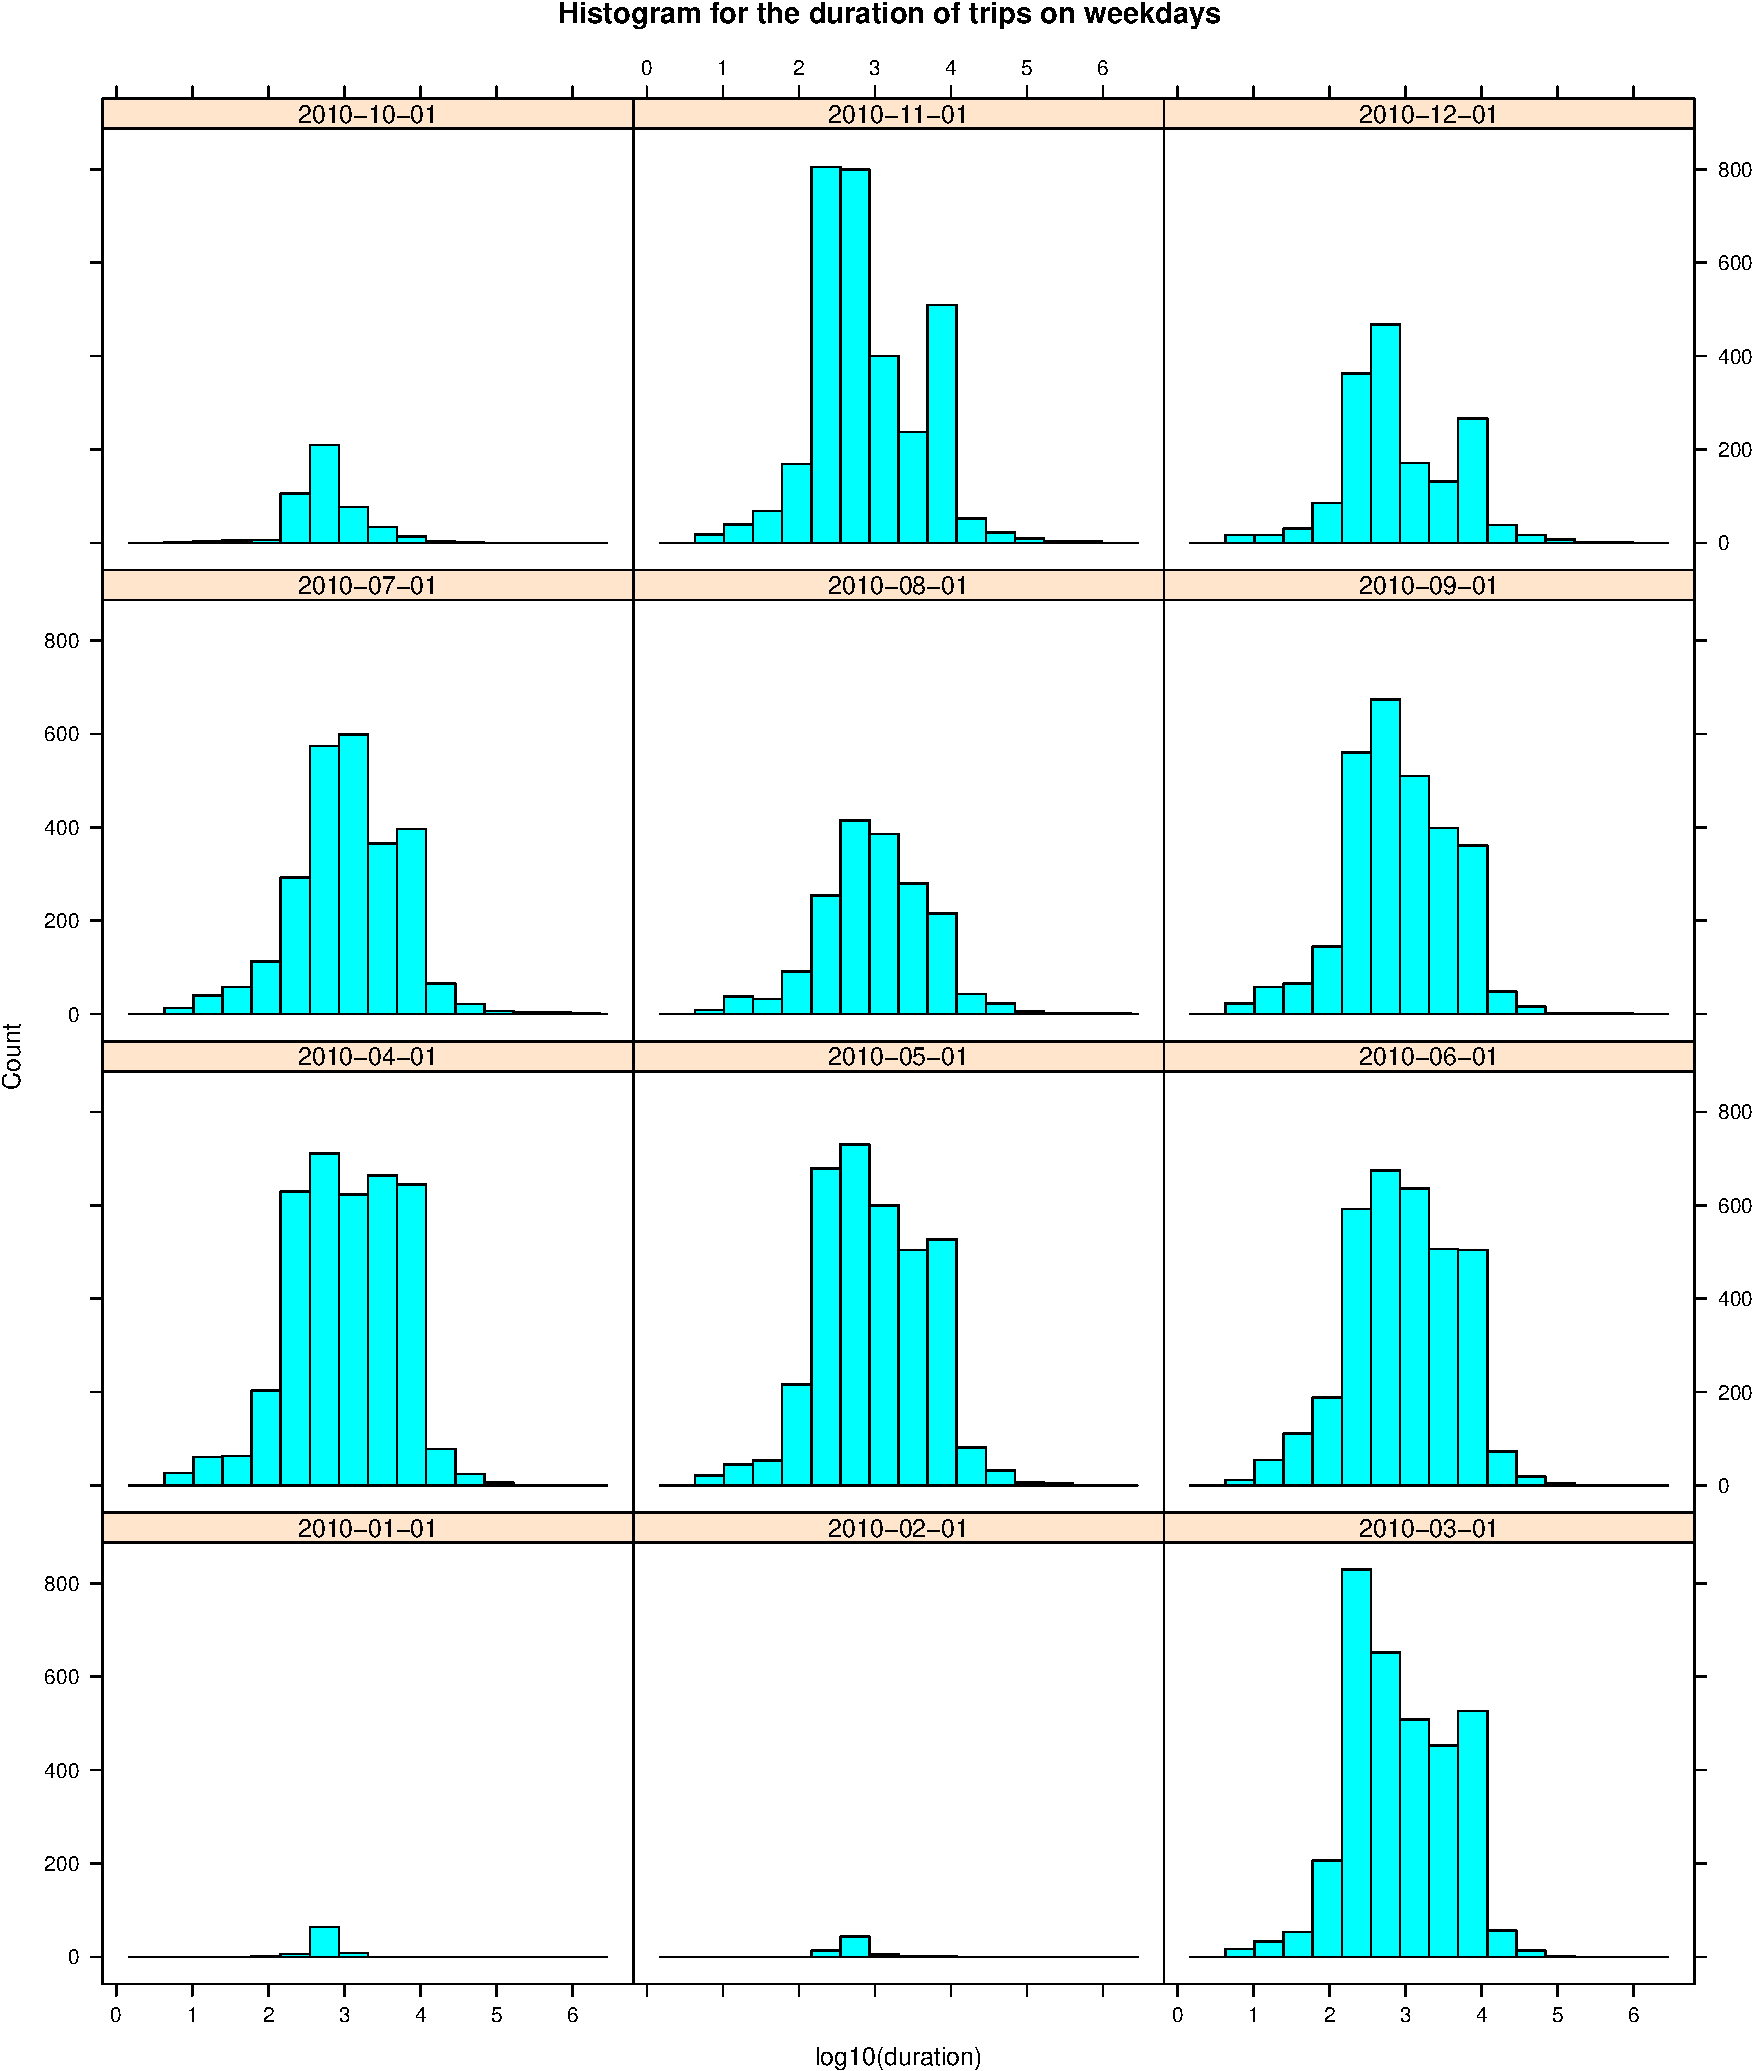
\includegraphics{velopassBirdsEye_files/figure-latex/tripdurations-2.pdf}
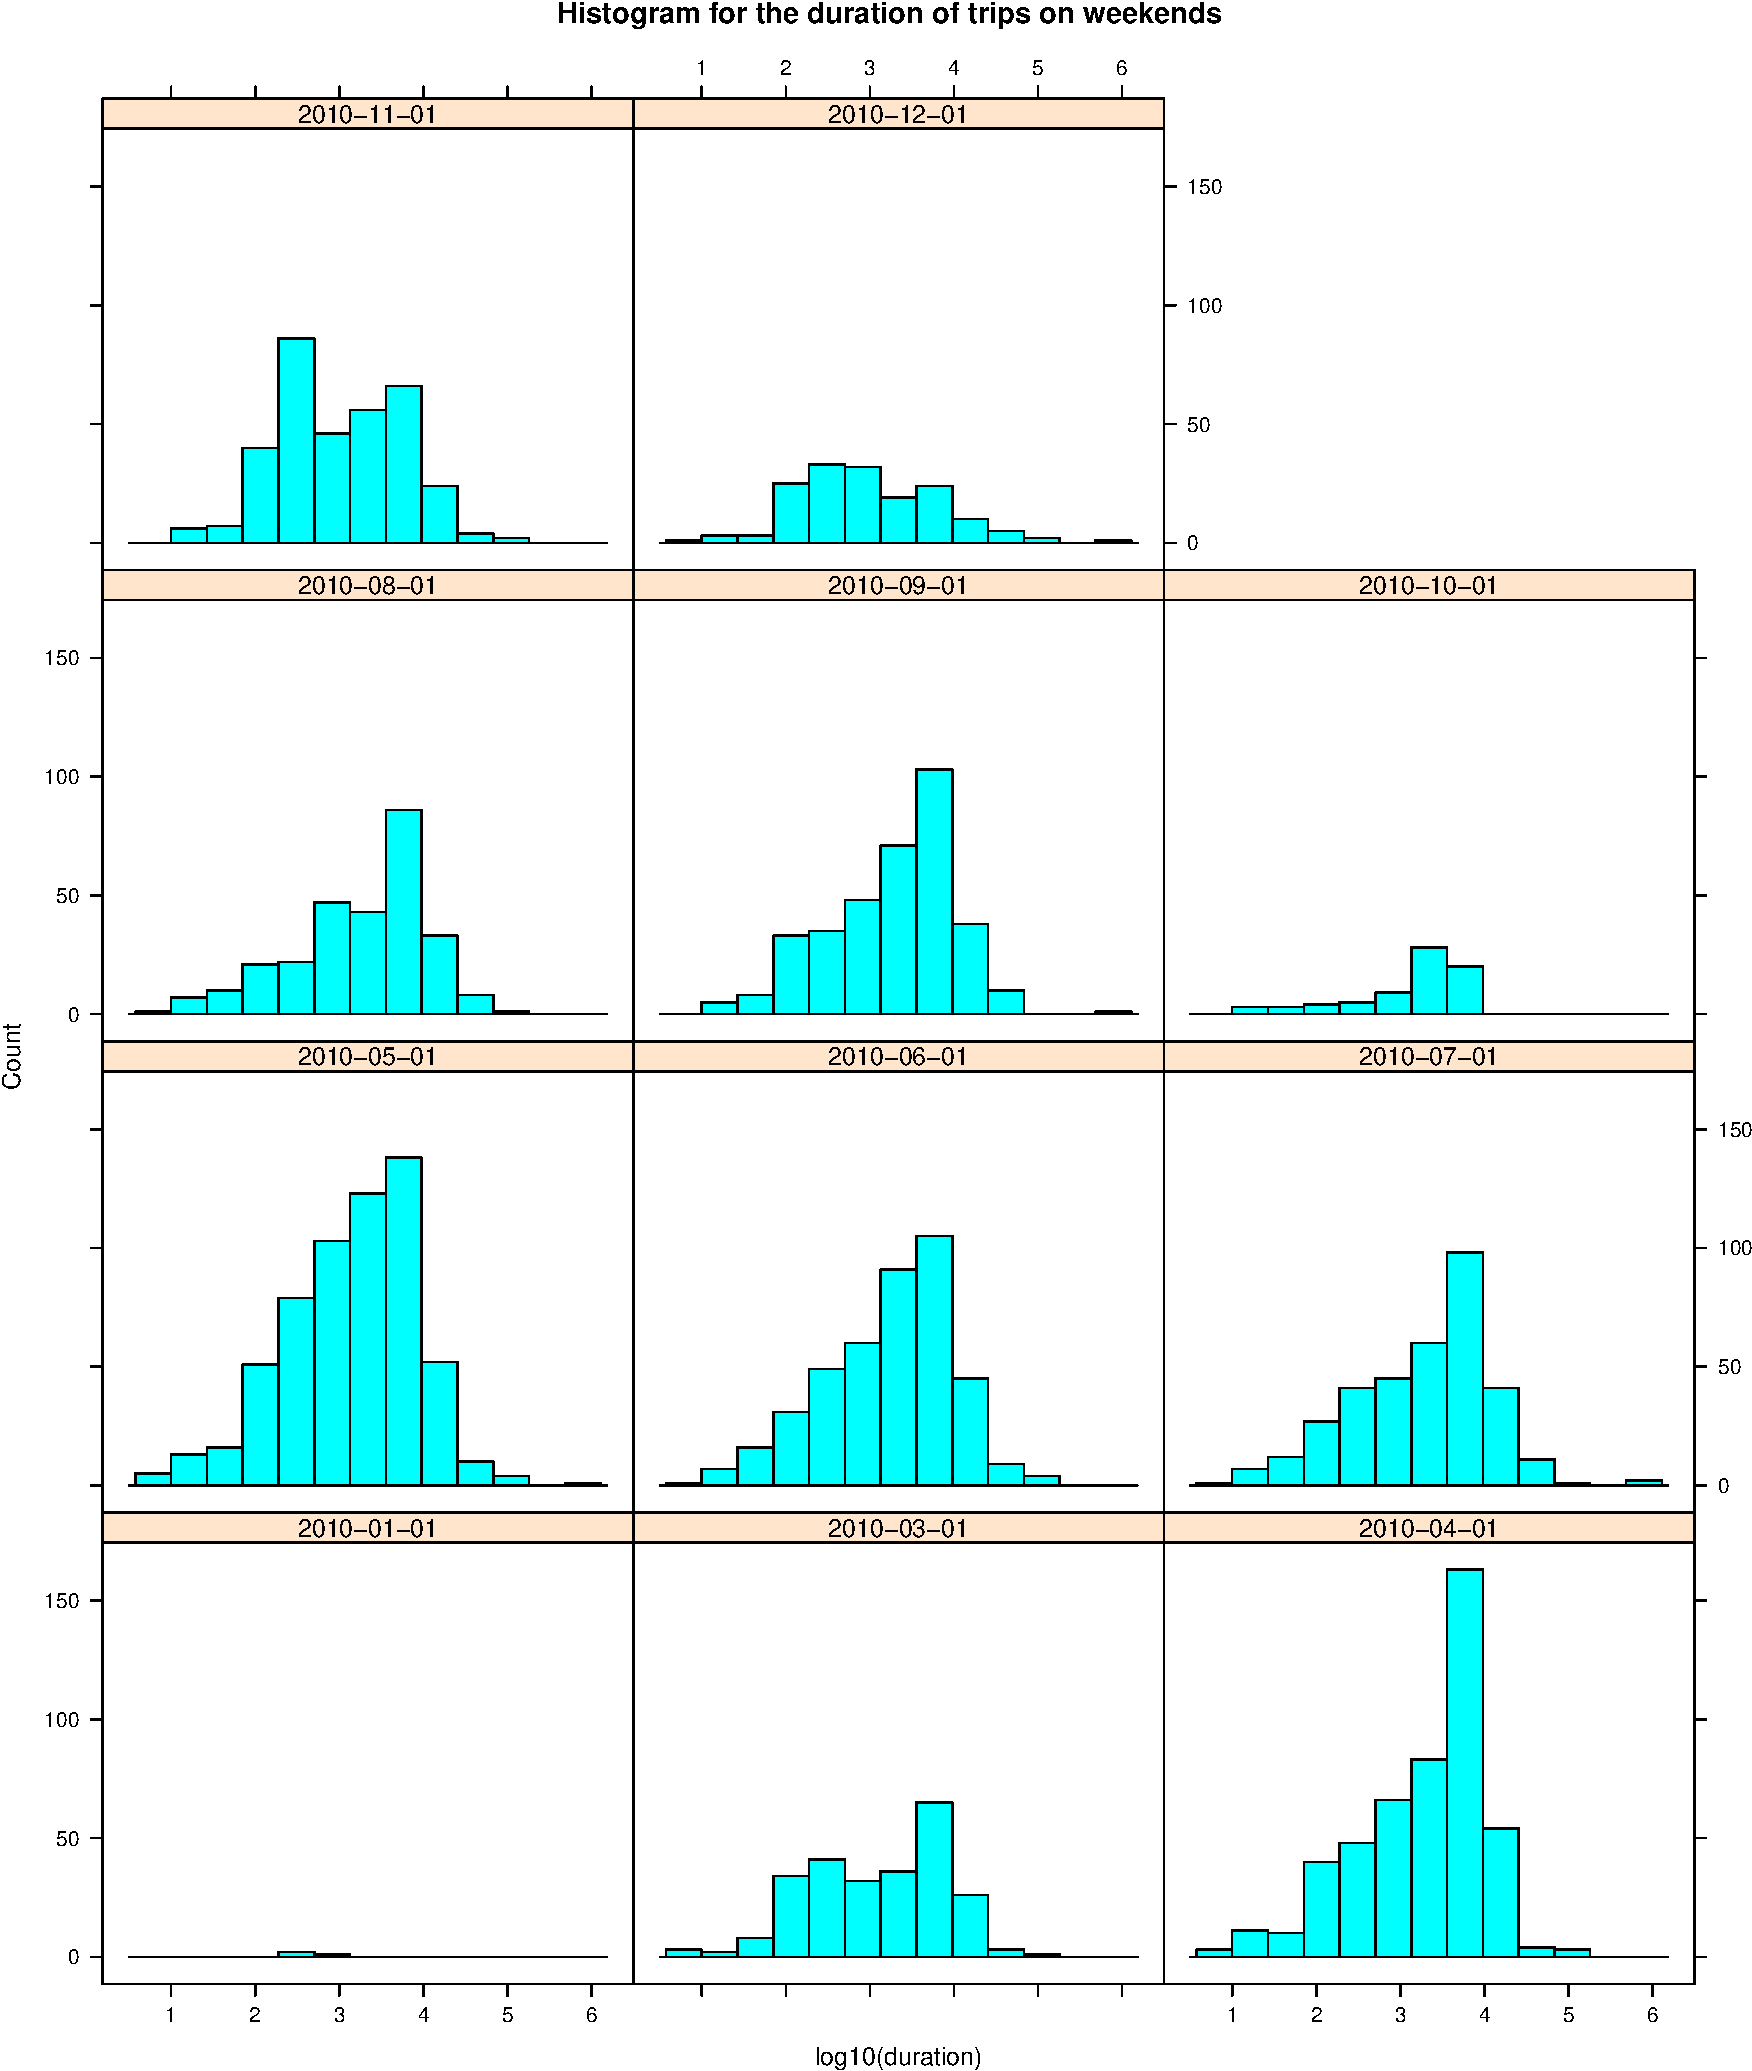
\includegraphics{velopassBirdsEye_files/figure-latex/tripdurations-3.pdf}

\subsection{Statistics for stations}\label{statistics-for-stations}

What stations are used most often?
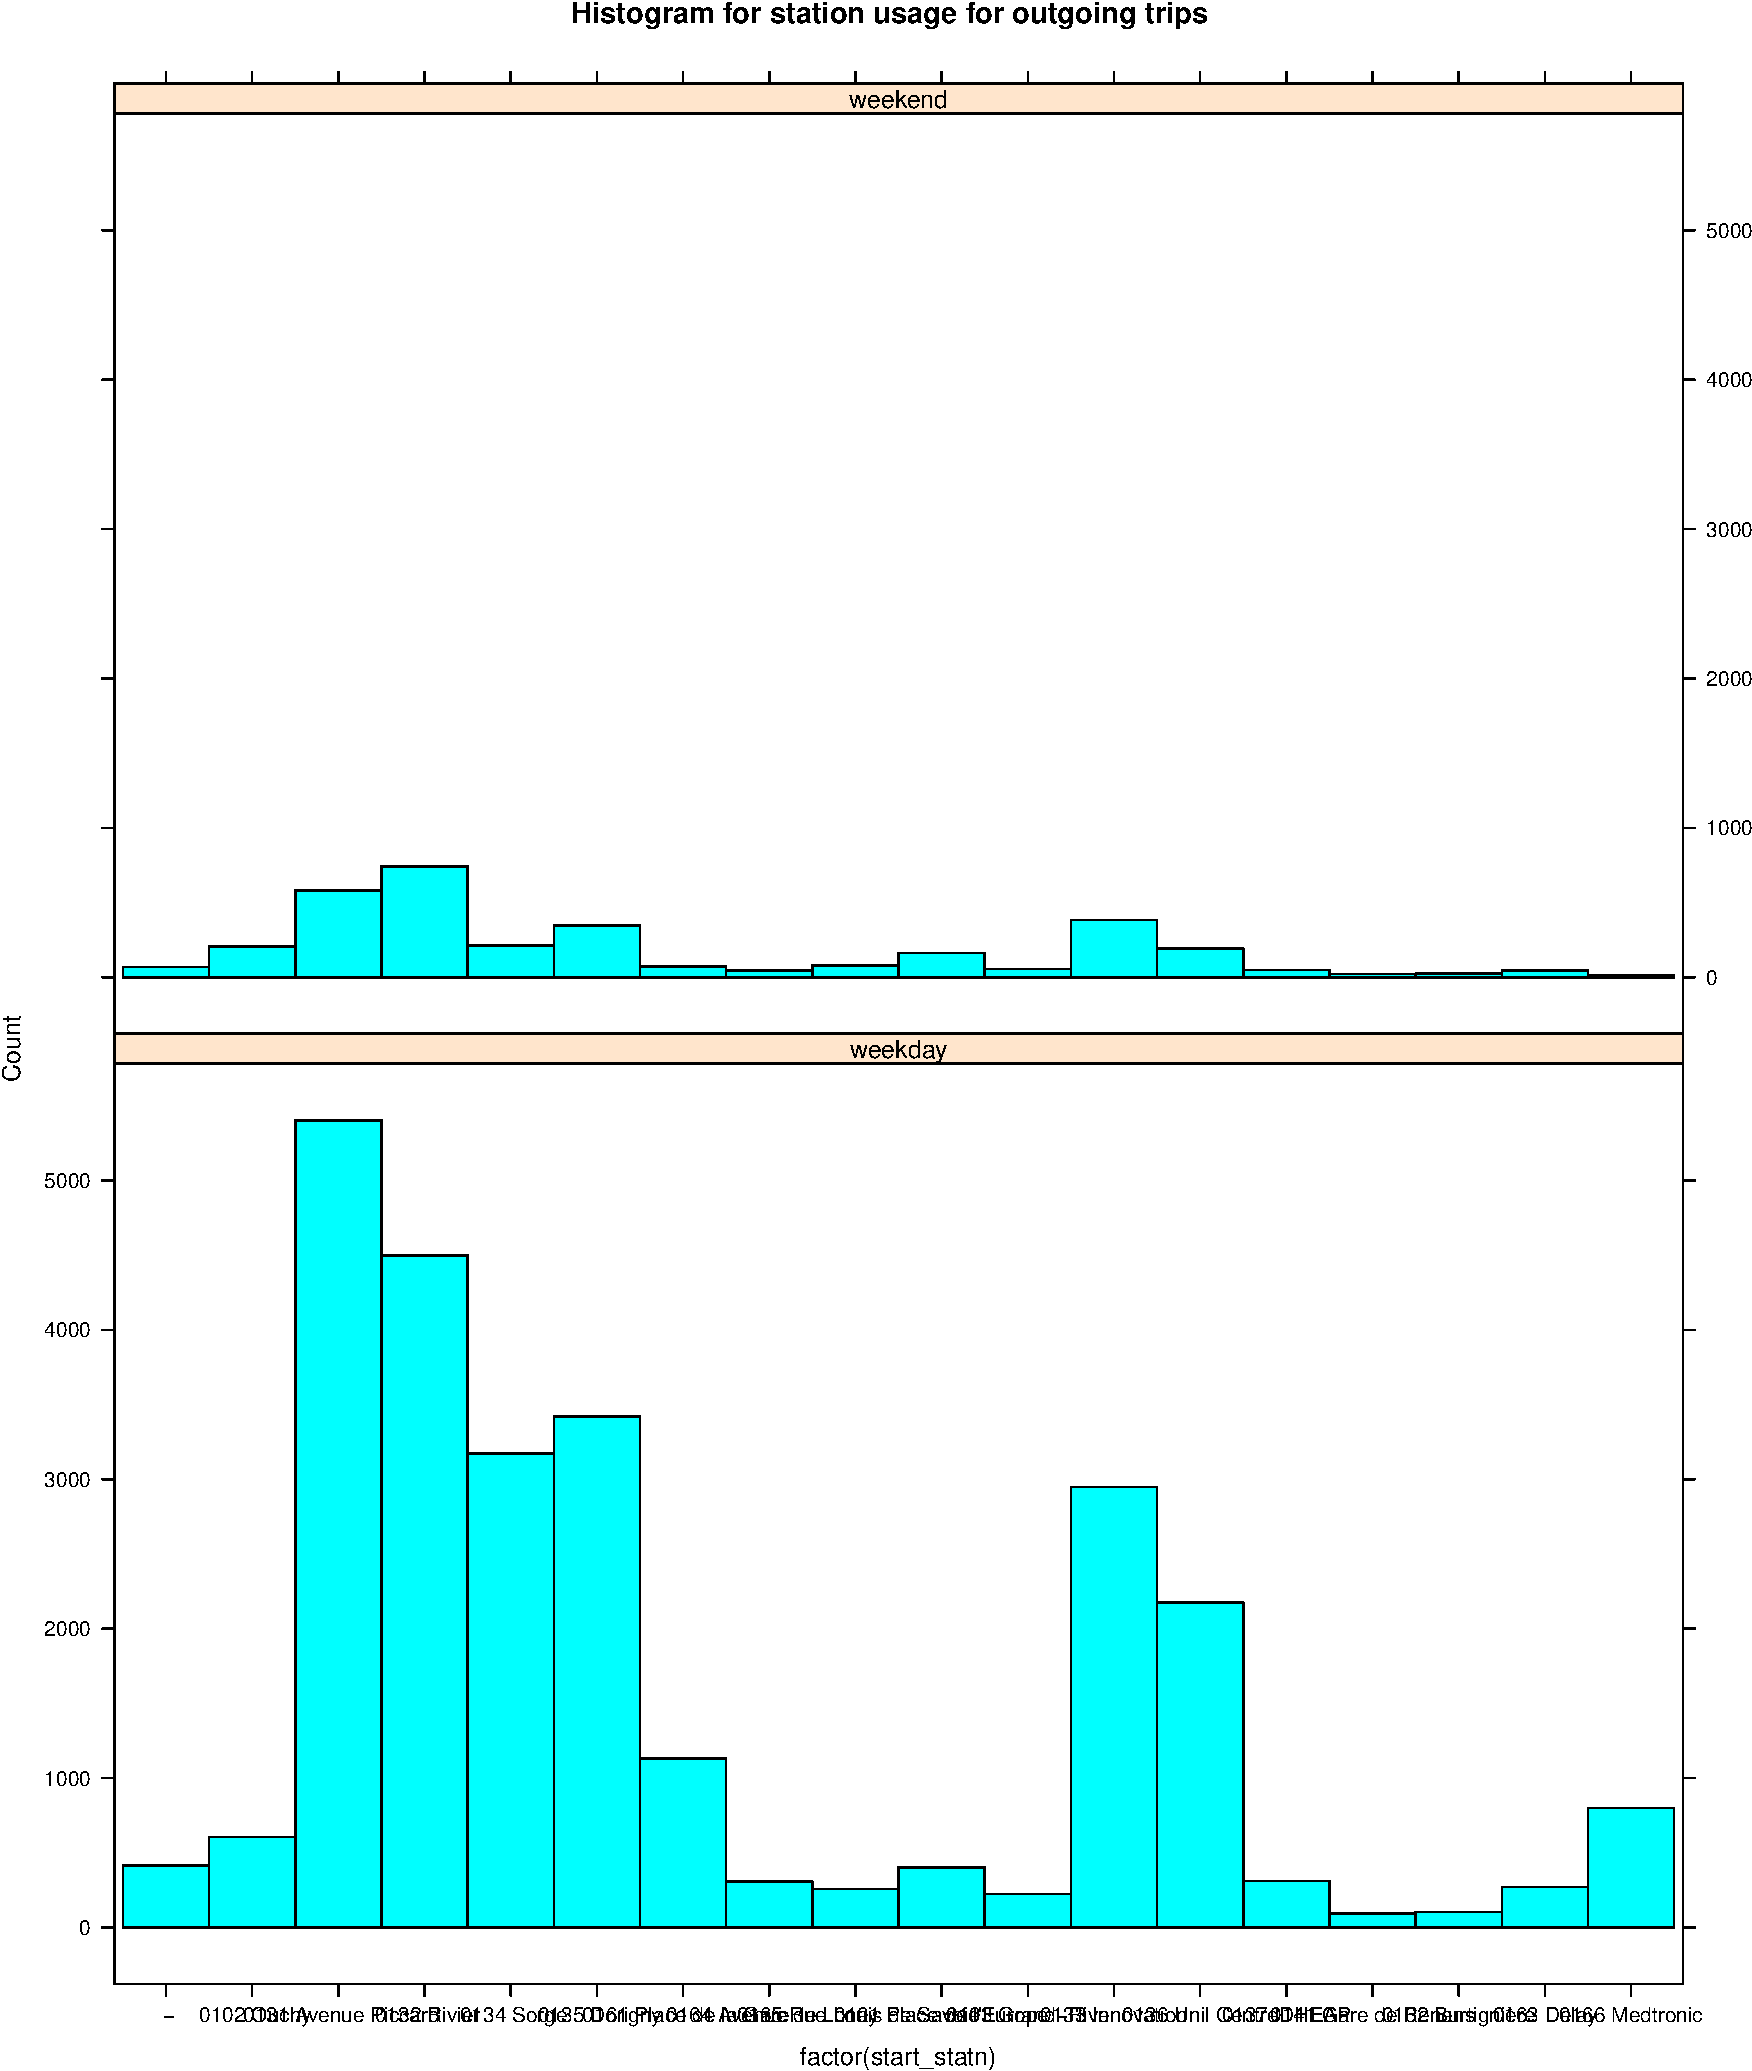
\includegraphics{velopassBirdsEye_files/figure-latex/stationUsage-1.pdf}
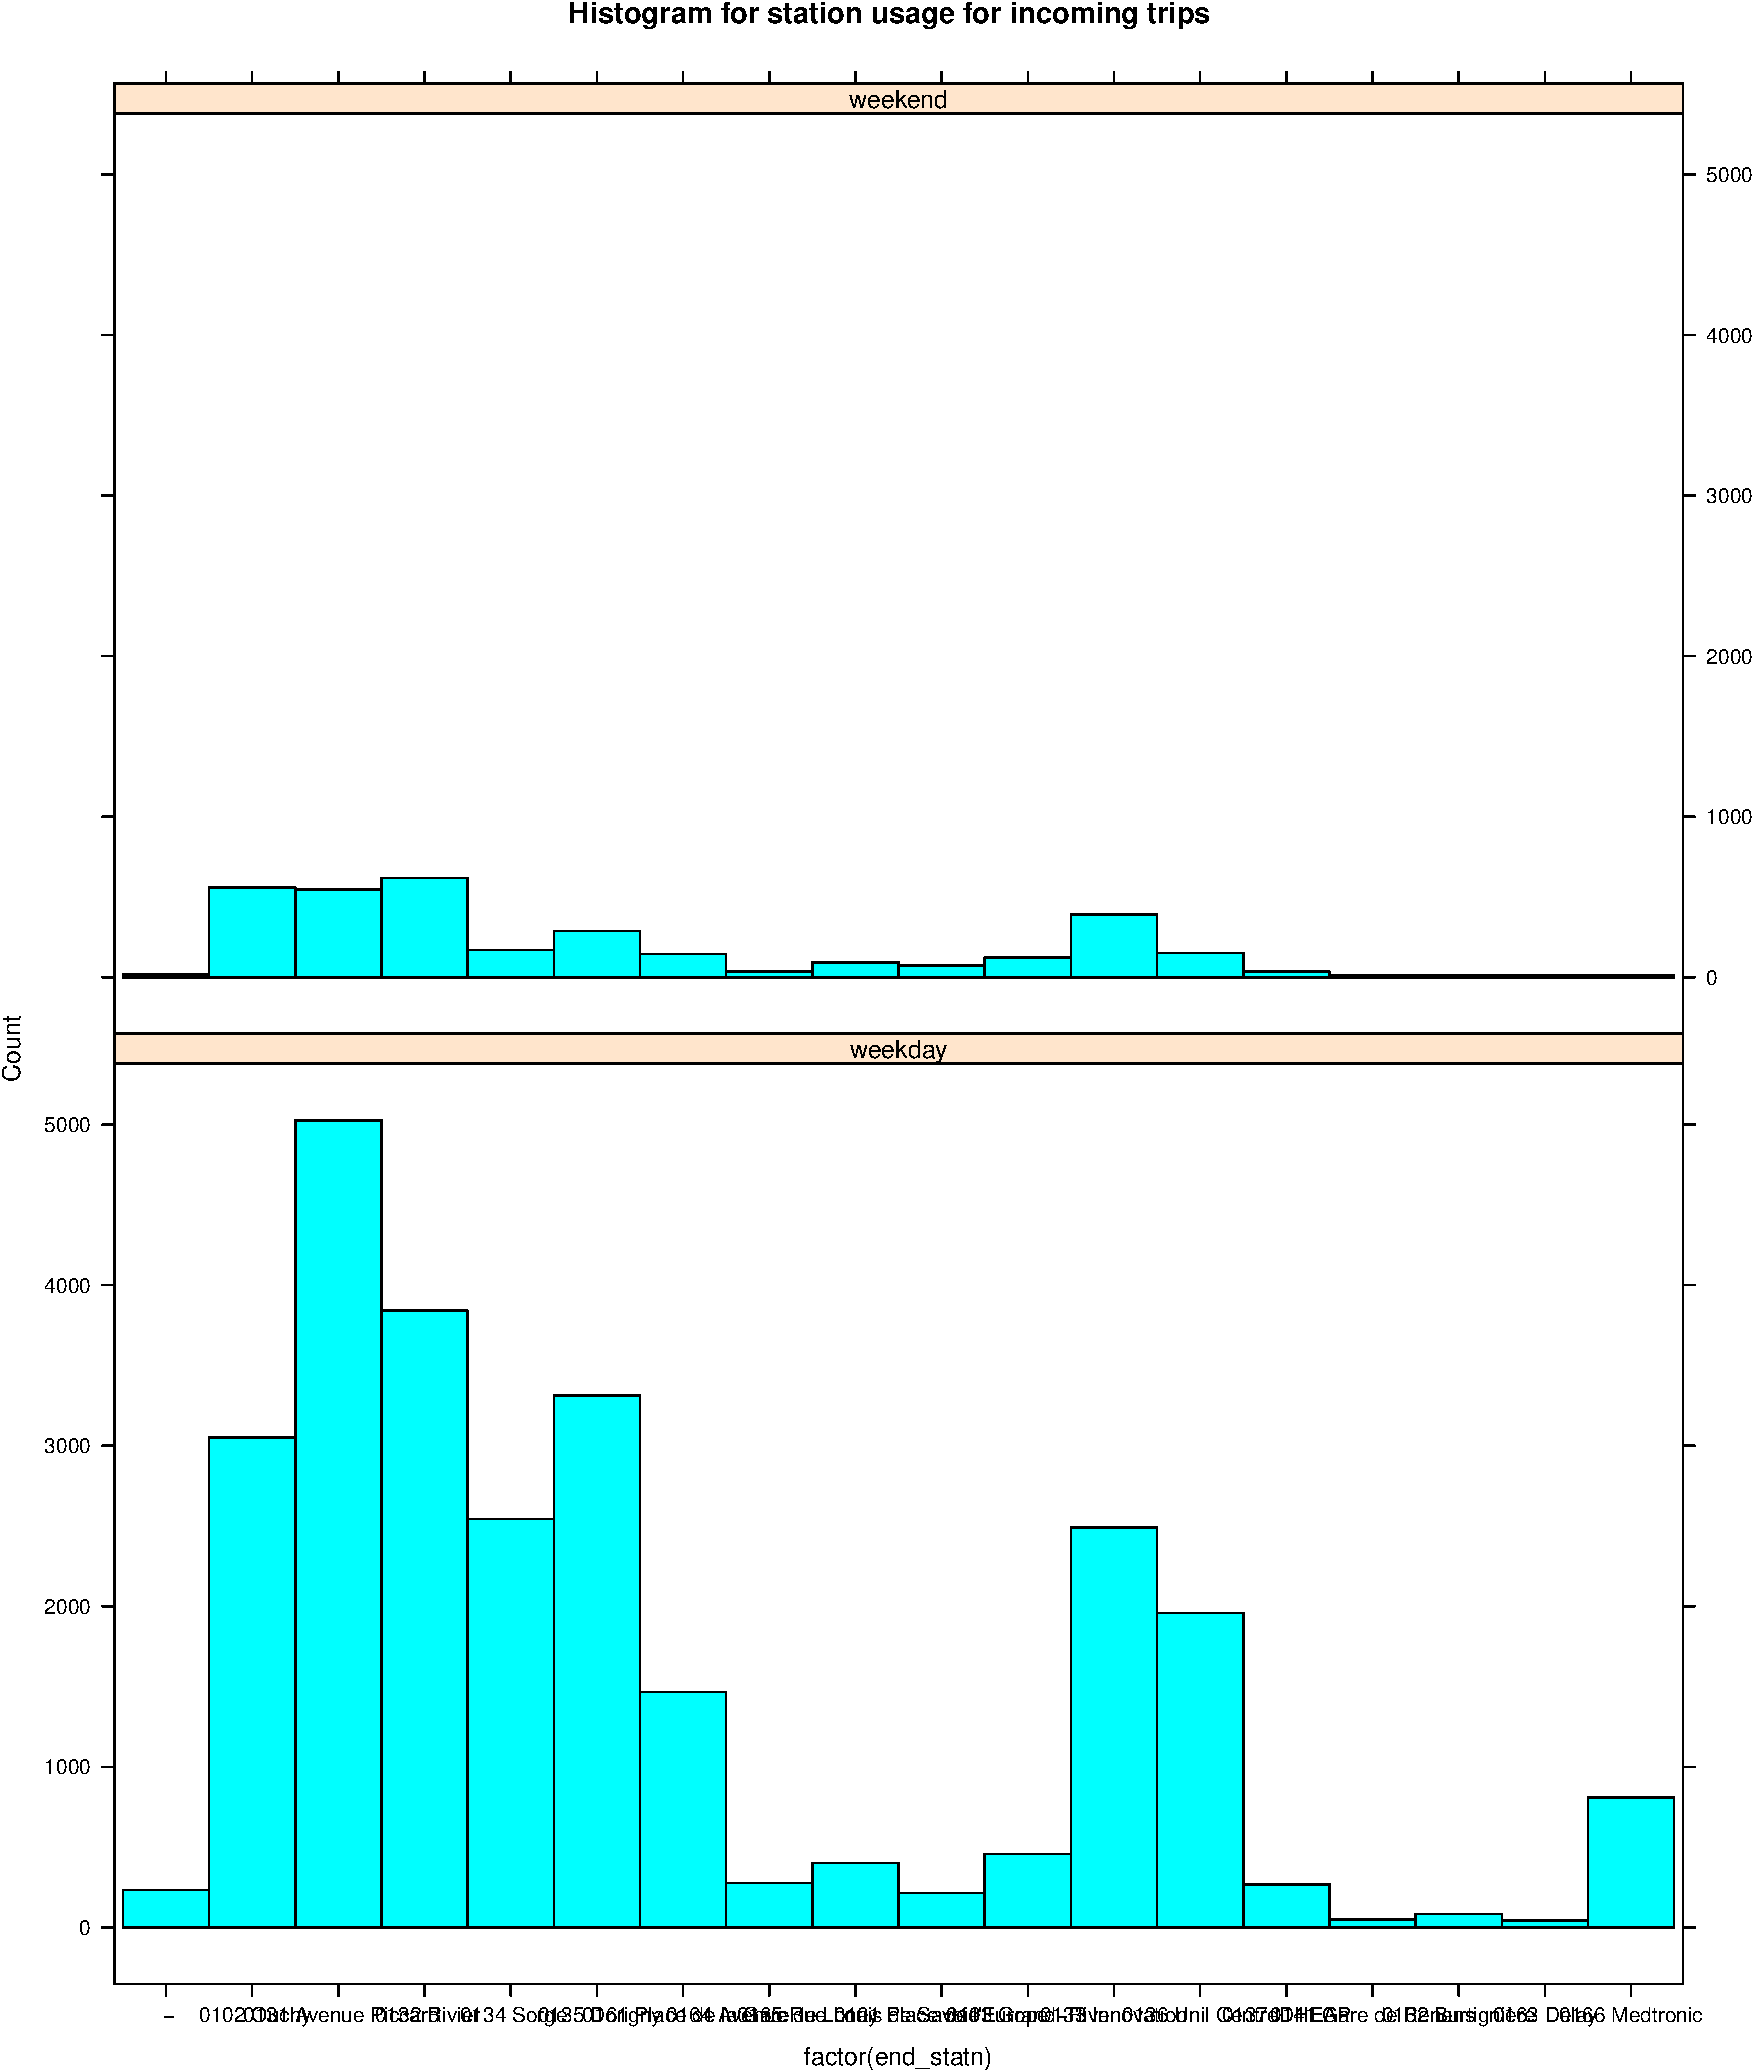
\includegraphics{velopassBirdsEye_files/figure-latex/stationUsage-2.pdf}

Individual station usage statistics is easy. We should also count the
number of stations between each pair of stations. For this we can make a
table.

\end{document}
